\documentclass[a4paper,twoside]{tufte-book}\usepackage[]{graphicx}\usepackage[]{color}
%% maxwidth is the original width if it is less than linewidth
%% otherwise use linewidth (to make sure the graphics do not exceed the margin)
\makeatletter
\def\maxwidth{ %
  \ifdim\Gin@nat@width>\linewidth
    \linewidth
  \else
    \Gin@nat@width
  \fi
}
\makeatother

\usepackage{Sweavel}

 %style file is in the same folder.

\usepackage[T1]{fontenc}
\usepackage[utf8]{inputenc}
%\usepackage{german}

\usepackage{color}
\usepackage{xcolor}
\usepackage{framed}
\usepackage{listings}

\usepackage{graphicx}

\usepackage{multicol}              
\usepackage{multirow}
\usepackage{booktabs}
%\usepackage{natbib} 

\usepackage[innerrightmargin = 0.7cm, innerleftmargin = 0.3cm]{mdframed}
\usepackage{mdwlist}

\usepackage[]{hyperref}
\definecolor{darkblue}{rgb}{0,0,.5}
\hypersetup{colorlinks=true, breaklinks=true, linkcolor=darkblue, menucolor=darkblue, urlcolor=blue, citecolor=darkblue}

\usepackage[toc,page]{appendix}


\setcounter{secnumdepth}{1}
\setcounter{tocdepth}{1}

\lstset{ % settings for listings needs to be be changed to R sytanx 
language=R,
breaklines = true,
columns=fullflexible,
breakautoindent = false,
%basicstyle=\listingsfont, 
basicstyle=\ttfamily \scriptsize,
keywordstyle=\color{black},                          
identifierstyle=\color{black},
commentstyle=\color{gray},
xleftmargin=3.4pt,
xrightmargin=3.4pt,
numbers=none,
literate={*}{{\char42}}1
         {-}{{\char45}}1
         {\ }{{\copyablespace}}1
}
% http://www.monperrus.net/martin/copy-pastable-listings-in-pdf-from-latex
\usepackage[space=true]{accsupp}
% requires the latest version of package accsupp
\newcommand{\copyablespace}{
    \BeginAccSupp{method=hex,unicode,ActualText=00A0}
\ %
    \EndAccSupp{}
}









\title{Grundlagen der\\Statistik}
\author{Florian Hartig}


\begin{document}
%\SweaveOpts{concordance=TRUE}
%\SweaveOpts{concordance=TRUE} % don't activate this for knitr

\let\cleardoublepage\clearpage % No empty pages between chapters
\maketitle


\thispagestyle{empty}
\null

\begin{fullwidth}
Vorlesungsunterlagen für Studierende der

\begin{itemize*}
  \item BSc Biostatistik
  \item MSc Research Skills (Webseite \href{http://florianhartig.github.io/ResearchSkills/}{hier})
\end{itemize*}

\vspace{0.5cm}

Anmerkungen / Fragen an:\\[0.5cm]
\href{https://florianhartig.wordpress.com/}{Florian Hartig}\\
Universität Regensburg\\
Germany\\[0.5cm]

Probleme oder Unklarheiten bei dieser Vorlesung können mittels \href{https://github.com/florianhartig/Statistics/issues}{issue tracker} der \href{https://github.com/florianhartig/Statistics/tree/master/EssentialStatistics}{GitHub repository} gemeldet werden. 

\end{fullwidth}


\vfill
\begin{fullwidth}
Erstellt 2014. Updated 2015. Diese Arbeit fällt unter die 'Creative Commons Attribution-NonCommercial- NoDerivatives 4.0 International' Lizenz.
\end{fullwidth}


\newpage
\tableofcontents

\chapter{Einleitung} % Use chapters instead of sections

	\section{Ziel und Zielgruppe diese Textes}
	
	Dieses Dokument beinhaltet eine kurze Einführung in die Statistik und in statistische Analysen, welcher es in elementaren Experimenten und beobachteten Situationen häufig bedarf~\ref{sec: further readings}.
	
	\section{Themen der Statistik und Datenwissenschaften}
	Statistik, oder auch Datenwissenschaften, behandelt die Visualisierung, Zusammenfassung und Interpretation von Daten. Dieses Skript beinhaltet eine Einführung in die vier wichtigsten Säulen der statistischen Methodik für einen quantitativen Wissenschaftler:
	
	\paragraph{Deskriptive Statistik:} Deskriptive Statistik\marginnote{Deskriptive Statistik = Plots, Kennzahlen der Statistik} beinhaltet die Kennzahlen der Statistik, wie beispielsweise der Mittel- oder Medianwert, aber auch weitere Optionen, um Daten zu visualisieren.
	
	\paragraph{Inferenzstatistik:} Inferenzstatistik\marginnote{Inferenzstatistik = Parameterschätzungen, p-Werte, Tests} behandelt das Testen von Hypothesen und Schätzen von Parametern. Inferenz basiert typischerweise auf Annahmen, welche in einem statistischen Modell zusammengefasst sind.\marginnote{Ein statistisches Modell beschreibt, wie Daten erstellt werden = Datenerzeugender Prozess} Ein statistisches Modell wird auch als "`datenerzeugender Prozess"' bezeichnet, da es Annahmen über einen Prozess beschreibt, die zu einer Variation an Daten führt (systematisch und stochastisch).
	
	\paragraph{Prädiktive Statistik und maschinelles Lernen:} Prädiktive Statistik und maschinelles Lernen\marginnote{Maschinelles Lernen = Vorhersagende Modelle. Große Dateien = umfangreiche Datensätze, z.\,B. von Amazon-Endkunden} arbeiten mit herleitenden Vorhersagen aus v.\,A. sehr "`großen Datensätzen"'. Der Hauptunterschied zur Inferenzstatistik ist, dass der Fokus auf der entstehenden Methode liegt, um gute Vorhersagen treffen zu können ohne ein vorhergehendes Beschreiben, Folgern oder Testen von Annahmen über den Datenerzeugenden Prozess.
	
	\paragraph{Experimentelle Planung:} Experimentelle Planung\marginnote{Experimentelle Planung oder Analysenplanung = das Erhalten und Erzeugen von Daten} umfasst alle Aspekte der Datenerzeugung, insbesondere Fragen wie "`Welche Variablen sollten erfasst werden?"', "`Wie viele Replikate werden benötigt?"', "`Wie sollten die Variablen in einem Experiment optimalerweise verändert werden?"'
	
	
	\section{Die Umgebung R für statistische Berechnungen}
	
	Die Zeiten als Statistik noch mit Stift, Papier und Taschenrechner durchgeführt wurde sind nun mehr oder weniger vorbei. Heutzutage werden statistische Analysen am Computer durchgeführt, wofür es eine Reihe von Software-Umgebungen gibt.
	
	In diesem Skript werden alle Beispiele mit Hilfe von R berechnet werden; wobei der Fokus jedoch nicht auf einer Einführung in R an sich liegen wird. Bei Bedarf führt  \href{http://biometry.github.io/APES/R/R10-gettingStarted.html}{dieser Link} zu einer Einführung, inklusive Hilfestellungen für die Installation der Software.
	
	\begin{figure}[]
		\begin{center}
			\includegraphics[width = 10cm]{rst_interface.png}
			\caption{Der RStudio Editor ist der wohl beliebteste Editor für R. R ist eine Script-basierende Sprache. Hier kommuniziert man nicht durch Klicken mit dem Computer, sondern gibt Anweisungen anhand von direkten Befehlen in der R Konsole, oder durch das vorhergehende Anlegen eines Text-Dokuments, welches dann die Befehle auswertet. Wenn man diese Herangehensweise nicht gewöhnt ist, kann es eine Weile dauern, bis man sich damit zurrecht findet. Wenn man sich jedoch damit angefreundet hat, wird man bald merken, wie komfortabel und vorteilhaft es ist, alle Schritte der Analyse in einem Textdokument aufgelistet wiederzufinden und somit alles zu jeder Zeit nachvollziehen zu können.}
			\label{fig: Rstudio}
		\end{center}
	\end{figure}
	
	
	
	\chapter{Daten, Proben und Populationen}
	
	Die folgenden vier Kapitel sind den vier Typen der statistischen Analyse zugewiesen, die in der Einleitung bereits genannt wurden: deskriptive Statistik, Inferenzstatistik, prädiktive Statistik und Versuchsplanung. 
	
	\section{Stichproben, Populationen und der Vorgang der Datenerzeugung}
	
	Der eigentliche Grund der für statistische Berechnungen spricht, ist, dass die Daten, die wir erhalten, sehr zufällig erscheinen. Aber wie entsteht diese Zufälligkeit?
	
	Man stelle sich vor, \marginnote{Eine Population ist die Zusammenstellung aller Beobachtungen, die man hätte machen können. Eine Stichprobe ist die Beobachtung, die man tatsächlich gemacht hat.} man wäre in die durchschnittliche Wachstumsrate der Bäumen in Deutschland während zwei aufeinanderfolgenden Jahren interessiert. Idealerweise sollte man alle Bäume per Hand messen und wäre somit ohne statistische Berechnungen ausgekommen. In der Praxis ist man jedoch kaum in der Lage dies durchzuführen. Um die durchschnittliche Rate ermitteln zu können, muss man nun eine Auswahl an Bäumen treffen und die Wachstumsrate aller dieser gewählten Bäume ermitteln. Der statistische Terminus für 'alle Bäume in Deutschland' lautet "`Population"' und die Bezeichnung der ausgewählten gemessenen Bäume ist "`Stichprobe"'.
	
	Die \marginnote{Das Wählen von Stichproben erzeugt Zufälligkeit.} Population an sich ist definiert und ändert sich nicht, jedoch könnte man bei jeder Untersuchung einer zufällig gewählten Stichprobe aus der Population andere Teilbereiche mit minimal unterschiedlichen Eigenschaften erhalten. Ein konkretes Beispiel: Man habe nur die Möglichkeiten um 1000 Bäume in Deutschland zu untersuchen. Man wird bei jeder zufällig gewählten Stichprobe mit 1000 Bäumen aus der gesamten Population unterschiedliche durchschnittliche Wachstumsraten erhalten.
	
	Der\marginnote{Jedoch kommt nicht jede Zufälligkeit durch das Wählen von Stichproben aus einer Population.} Vorgang des Stichproben-Festlegens aus einer Population erklärt, wie die Zufälligkeit in unseren Daten entsteht. Jedoch gibt es ein kleines Problem bei dieser überlegung, da dies nicht immer zutrifft, wenn man beispielsweise komplexere Zufallsprozesse betrachtet. Man gehe exemplarisch davon aus, dass man Daten z.B. durch eine Person erhält, welche zu zufällig ausgewählten Punkten geht und daraus die Ausbreitung ermitteln möchte (welche innerhalb von Minuten durch wechselnde Bewölkung variieren kann). Man verwendet dazu ein Messgerät, das mit zufälliger Abweichung misst. Macht es da wirklich Sinn auf Daten zu vertrauen, die durch das Stichproben-Wählen aus einer Gesamtpopulation mit verschiedenst möglichen Beobachtungen entstanden sind?
	
	\marginnote{Eine modernere und allgemeinere Idee, welche das potentielle Entstehen von Daten beschreibt, ist das Konzept des "`datenerzeugenden Vorgangs"', wobei der Name bereits verrät, was dahinter steckt: der datenerzeugende Vorgangs beschreibt, wie die Beobachtung einer zufällig gewählten Stichprobe entsteht und dabei zusätzlich systematische und stochastische Prozesse mit einbezieht.}  Dafür bezieht es die Eigenschaften mit ein, welche typischerweise als "`Stichprobenerhebung aus der Population"' bezeichnet werden, jedoch dies in umfassenderen Ausmaß, indem es all die anderen Vorgänge, die systematische und zufällige Muster im Datensatz entstehen lassen können, einschließt. In diesem Fall schlussfolgert man nicht die Umstände der Population aus der Stichprobe, sondern wir würden die Umstände des datenerzeugenden Prozesses aus den Stichproben-Beobachtungen, die durch diesen Prozess entstanden sind, schließen. 
	
	Egal, ob man in Populationen oder datenerzeugenden Prozessen denkt: Das Essenzielle aus diesem Abschnitt ist, dass es zwei Objekte gibt, die man strikt unterscheiden soll: zum Einen gibt es unsere Stichprobe. Man beschreibt sie meist durch ihre Zustände (Mittelwert, Minimum, Maximum), jedoch ist eine Stichprobe nicht das eigentliche Ziel. Letztendlich möchte man lediglich die Umstände der Population / des datenerzeugenden Prozesses aus der Stichprobe schlussfolgern. Dazu kommen wir im nächsten Abschnitt der Inferenzstatistik. Davor müssen wir jedoch noch einen genaueren Blick auf die Darstellung von Stichproben, beziehungsweise auf die Tatsachen, die wir beobachten, werfen.
	
	\section{Darstellung und Datenklassen}
	
	Ein typischer Datensatz beinhaltet meist mehrere Beobachtungen von verschiedensten Variablen (z.B. Temperatur, Niederschlag, Wachstum). Man kann sich dabei eine Tabelle vorstellen, in der die Spalten die Variablen bezeichnen und die Reihen die unterschiedlichen Beobachtungen. Natürlich gibt es auch andere Datenstrukturen, jedoch ist diese die wohl Häufigste.
	
	üblicherweise enthalten die Daten eine Variable auf der unser Fokus liegt, d.h. wir möchten herausfinden, wie sehr unsere Variable von den anderen Variablen beeinflusst wird. \marginnote{Die Response-Variable ist die Variable, für die wir herausfinden wollen, inwiefern sie von anderen Faktoren abhängt.}  Diese Variable wird als ``Response-Variable'' bezeichnet (manchmal auch abhängige Variable oder Ergebnisvariable), da wir wissen wollen, ob und wie diese untersuchte Variable variiert (Reaktion, Abhängigkeit) wenn sich etwas anderes verändert. Diese anderen Variablen, die unsere untersuchte Variable beeinflussen, können unter anderem Umweltfaktoren (z.B. Temperatur) oder Behandlungen (befruchtet vs. unbefruchtet) sein. \marginnote{Einflussvariablen sind solche, die die Response-Variable beeinflussen.} Diese anderen Variablen, die unsere untersuchte Variable beeinflussen, nennt man "`Einflussvariablen"' (Synonyme hierfür wären erklärende Variablen, Kovariaten oder unabhängige Variablen). 
	
	In den \marginnote{Multivariate Statistik behandelt Response-Variablen mit mehreren Dimensionen, wie z.B. Artenzusammensetzungen} meisten Fällen ist unsere Response-Variable eine einzelne Variable (beispielsweise eine einfache Zahl oder ein kategorisches Ergebnis), worauf wir uns nun konzentrieren. Manchmal gibt es jedoch Fälle, bei denen eine Response mehr als nur eine Dimension einnimmt, oder wenn man an einer Veränderung von mehreren Variablen gleichzeitig interessiert ist. Das Auswerten solcher Daten wird als multivariate Statistik bezeichnet. Diese Methoden werden jedoch hier nicht weiter aufgeführt, können aber bei Bedarf unter diesem \href{http://biometry.github.io/APES/Stats/stats50-MultivariateStatistics.html}{Link} nachgelesen werden.
	
	Weiterhin ist zu beachten, dass man die Variablenart unterscheiden muss; unabhängig davon, ob wir von Response- oder Einflussvariablen sprechen. Man unterscheidet hier: \marginnote{Variablen können stetig, unstetig oder kategorisch sein. Kategorische Variablen können geordnet, ungeordnet oder binär sein.}
	
	\begin{itemize}
		\item Stetig numerische Variablen (geordnet und stetig / real), z.B. Temperatur
		\item Ganzzahlig numerische Variablen (geordnet, ganzzahlig). Hierzu zählt der wichtige Spezialfall der Zähldaten, z.B. 0,1,2,3, ...
		\item Kategorische Variablen (z.B. eine feststehende Auswahlmöglichkeit wie beispielsweise rot, grün, blau), welche dann weiterhin unterteilt werden können in 
		\begin{itemize}
			\item Ungeordnete kategorische Variablen (nominal) wie beispielsweise rot, grün, blau
			\item Binäre (dichotome) Variablen (verstorben / überlebt, 0/1)
			\item Geordnete kategorische Variablen (klein, mittel, groß)
		\end{itemize}
	\end{itemize}
	
	Hier ist es äußerst wichtig die Variablen ihren entsprechendem "`Typ"' zuzuweisen.\marginnote{Man muss überprüfen, ob die Variablen zum richtigen Typ zugewiesen wurden, nachdem man sie in das Statistikprogramm eingegeben habt.} Und falls man eine Statistik-Software benutzt, muss man sicher stellen, dass der Typ auch korrekt erkannt wurde, nachdem die Daten eingegeben wurden, da viele Methoden die Variablen unterschiedlich behandeln, wenn sie numerischem oder kategorischem Typs sind.
	
	Aus Erfahrung weiß man, dass Anfänger eher dazu neigen, Variablen als kategorisch einzuordnen, obwohl diese eigentlich stetig wären, z.B. beim Einteilen von Körpergewicht von Tieren in leicht, mittel und schwer.\marginnote{Verwende nie kategorische Variablen für Dinge, die ebenso als numerisch eingestuft werden können!} Eine Rechtfertigung dafür ist meist, dass es ein ungewisses Messen vermeidet. Kurz gesagt: Das tut es ganz und gar nicht.Es ruft nur zusätzliche Probleme hervor. Verwende nie kategorische Variablen für Dinge, die ebenso als numerisch eingestuft werden können!
	
	
	\vspace{1cm}
	\begin{fullwidth}
		\begin{mdframed}
			
			\textbf{In R:} 
			
			Um Daten darzustellen besitzt R eine grundlegende Datenstruktur, den Daten-Frame (data.frame). Ein Daten-Frame ist gleichzusetzen mit einer Tabelle mit Spalten, wobei jede Spalte einen anderen Typ haben kann. Möglichkeiten hier sind
			
			\begin{itemize*}
				\item ganzzahlig - selbsterklärend
				\item numerisch - kontinuierliche Nummern (Gleitkommazahl)
				\item boolean (=aussagenlogisch) - true / false
				\item Faktor - normalerweise ungeordnet, z.B. rot, grün, blau. Kann auch geordnet sein (klein, mittel, groß), wobei es hier manchmal ratsam wäre, diese als ganzzahlig einzustufen
			\end{itemize*}
			
			Desweiteren gibt es den Fall der ausbleibenden Beobachtung einer Variablen, auch wenn dies nicht wirklich ein Datentyp ist. Dies wird dann typischerweise mit "`NA"' betitelt. ähnlich, jedoch nicht identisch ist "`NaN"' (not a number), was bei einer nicht ausführbaren Rechnung als Ergebnis auftreten kann.
			
			Um Daten als data.frame in R-studio einzulesen, findet man im oberen rechten Teil "Import Dataset". Genaueres kann unter "Handling data in R " im Anhang~\ref{HandlingDataInR}, oder auf \href{http://biometry.github.io/APES/R/R20-DataStructures.html}{der Seite hier} nachgelesen werden.
			
			Nachdem die Daten eingelesen wurden, ist es sehr wichtig die Spalten auf ihre richtigen Typen zu überprüfen. Dies wird ausgeführt durch str(TheNameOfMyData), womit man kann die Spalten auf ihre Typen checken kann.
			
		\end{mdframed}
	\end{fullwidth}
	
	
	\chapter{Deskriptive Statistik und Visualisierung}
	
	Deskriptive Statistik\marginnote{Wie man Daten erstellt wird später noch detaillierter im Kapitel ~\ref{cha: design of experiments} Versuchsplanung behandelt.} behandelt die Zusammenfassung und Veranschaulichung von (die durch Stichproben gewählten) Daten
	
	\section{Kennzahlen der Statistik}
	
	Kennzahlen der Statistik\marginnote{Kennzahlen der Statistik fassen die Daten zusammen} sind numerische Berechnungen, die Datensätze zusammenfassen. Dies dient zur kompakten Veranschaulichung der Eigenschaften eines Datensatzes.
	
	\subsection{Zusammenfassen einer einzelnen stetigen Variable}
	
	Eine übliche Situation bei der wir von den Kennzahlen der Statistik Gebrauch machen, ist die wiederholte Beobachtung einer stetigen Variable. Als Beispiel kann man sich hier vorstellen, man habe 2000 Bäume gemessen und anschließend erneut vermessen. Man konnte eine Vorkommen an zunehmendem Durchmesser beobachten (siehe Abb.\ref{fig: data distribution}).

\begin{figure}[htbp]
\begin{center}
\begin{Schunk}

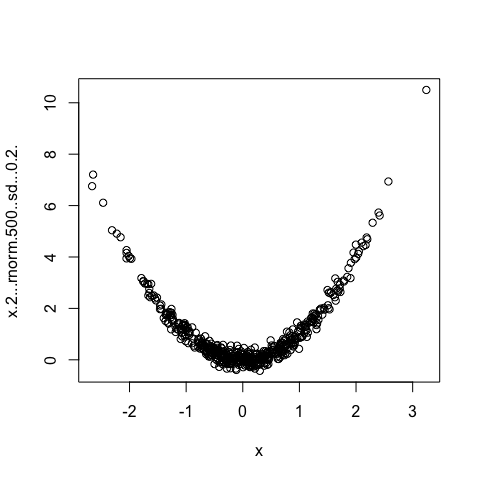
\includegraphics[width=\maxwidth]{figure/unnamed-chunk-2-1} \end{Schunk}
\caption{Eine Verteilung von beobachteten zunehmenden Durchmessergrößen (graue Balken). Wir nehmen an (in diesem Fall wissen wir es), dass diese Werte von wahren Verteilungen stammen (Population oder datenerzeugender Prozess) die hier in einer rot-gestrichelten Linie angedeutet werden. Wenn wir nun mehr Daten aufzeichnen würden, würden sich die grauen Balken der wahren Verteilung immer mehr annähern.}
\label{fig: data distribution}
\end{center}
\end{figure}

Wie kann man nun die Eigenschaften der beobachteten Stichprobe zusammenfassen? Ein paar grundlegende Eigenschaften wären beispielsweise das Minimum und das Maximum, der Mittelwert, oder der Modalwert (die Maximalverteilung, d.h. der Wert der höchsten Beobachtungsdichte). Außerdem  gibt es zwei weitere Kennzahlen, die ebenso oft Gebrauch finden: Moment und Quantil.


Der Begriff "`Moment"' mag vielleicht nicht jedem geläufig sein, vermutlich wurde aber schon einmal das erste und zweite Moment der Verteilung berechnet. Diese sind ebenfalls unter den Bezeichnungen Mittelwert und Standardabweichung bekannt. Allgemein wird das n-te Moment $\mu_n$ einer Verteilung $f(x)$ um einen Wert c definiert als 

\begin{equation}
\mu_n(c) = \int_{-\infty}^{\infty} f(x) (x - c)^n dx
\end{equation}

oder, für eine endliche Anzahl an Beobachtungen 

\begin{equation}
\mu_n(c) = \frac{1}{N}\sum_{i=1}^N (x_i - c)^n dx
\end{equation}

Das erste Moment mit c=0, ist der Mittelwert. Für die folgenden höheren Momente ist es üblich die Zentralmomente zu betrachten, die man durch das Setzen von c auf den Mittelwert erhält, da ihre Werte einfacher als Indikatoren für die Verteilungsform zu interpretieren sind.\footnote{Um die Varianz abzuschätzen, ersetzt man oft den Term 1/N durch den Bias-korrigierten Term 1/(N-1).} Die drei höheren Zentralmomente werden Varianz (n=2, identisch mit dem Quadrat der Standardabweichung, Messgröße der Streuung), Schiefe (n=3, Messgröße für die Asymmetrie in der Verteilung) und Wölbung (n=4) genannt. 

Quantilen stellen die zweite Zentralklasse der Kennzahlen-Statistik dar, um die kontinuierliche Verteilung zu beschreiben. Wenn wir eine Verteilung wie in der oben gezeigten Abbildung vorfinden, kann man sich die Frage stellen: Welcher ist der entscheidende Wert, der den Datensatz in zwei Hälften trennt, sodass eine Hälfte der beobachten Daten kleiner und die andere Hälfte größer als dieser Wert ist?\marginnote{Eine Hälfte der Daten ist kleiner und die andere Hälfte ist größer als die 0.5 Quantile, welches auch als Medianwert bezeichnet wird} Dieser Punkt wird als Medianwert, oder auch als 0.5-Quantil bezeichnet. Allgemeiner kann man sagen, dass die 0.x Quantile der Wert ist, an dem der Anteil 0.x des Datensatzes kleiner ist. 

\subsection{Korrelation - Erläuterung der Abhängigkeit stetiger Variablen}

Ein weiterer wichtiger Bereich der Kennzahlen-Statistik ist die Korrelation. Korrelationsstudien messen die Abhängigkeit von stetigen Variablen. Leider gibt es eine Menge Korrelations-Messgrößen, die es zu unterscheiden gilt. Die zwei wichtigsten sind:

\paragraph{Lineare Koeffizienten:}Lineare Koeffizienten, mit dem "`Pearson'schen Korrelationskoeffizienten"', als dem wohl Häufigsten, ermitteln die lineare Abhängigkeit zwischen zwei Variablen. Der Pearson'sche Korrelationskoeffizient wird wegen seiner schnellen Berechnung und leichten Interpretation am häufigsten verwendet. Jedoch kann es hier zu Fehlern kommen, wenn die Variablen nicht linear abhängig voneinander sind. Fig.~\ref{fig: correlation}.

\paragraph{Rangkorrelationskoeffizient:} Rangkorrelationskoeffizient, wie zum Beispiel der "`Spearman'sche Rangkorrelationskoeffizient"' und der "`Kendall Tau Rangkorrelationskoeffizient"' ermitteln, wie genau die Variablen gemeinsam tendenziell steigen oder fallen, ohne hierbei das Ausmaß oder die Linearität ihrer Steigung zu beachten. Diese werden bevorzugt, wenn man von zueinander nicht-linearen Variablen ausgeht. 

\paragraph{Starke Korrelation != bedeutender Einfluss:} Siehe auch Fig.~\ref{fig: correlation}; ist ein oft falsch verstandener Zustand der Korrelation und Abhängigkeit - ein hoher Korrelationskoeffizient bedeutet nicht, dass eine Variable eine starke Reaktion auf eine andere bewirkt. Um eine hohe Korrelation zu erreichen braucht es nur eine geringe Streuung um die Korrelationslinie (siehe mittlere Reihe - die Auswirkung ist anders, aber die Korrelation bleibt gleich). 


\begin{figure}[htbp]
\begin{center}
\begin{Schunk}
\begin{Soutput}
Error in library(mvtnorm): there is no package called 'mvtnorm'
\end{Soutput}
\begin{Soutput}
Error: konnte Funktion "rmvnorm" nicht finden
\end{Soutput}
\begin{Soutput}
Error in RotNormal(200, c(0, pi/12, pi/6, pi/4, pi/2 - pi/6, pi/2 - pi/12, : konnte Funktion "rmvnorm" nicht finden
\end{Soutput}
\begin{Soutput}
Error in Others(800): konnte Funktion "rmvnorm" nicht finden
\end{Soutput}

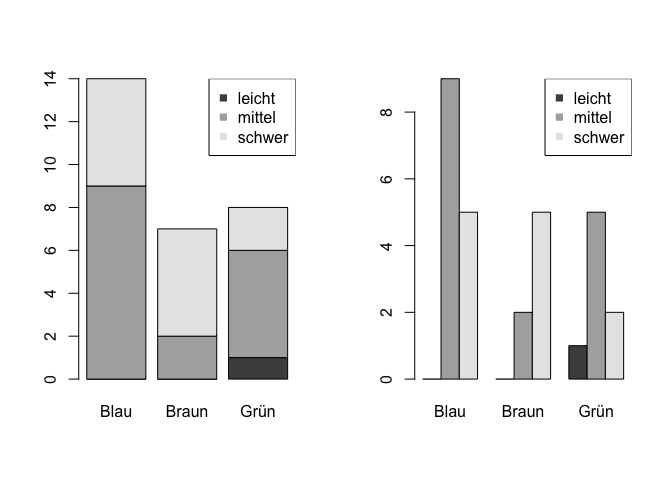
\includegraphics[width=\maxwidth]{figure/unnamed-chunk-3-1} \end{Schunk}
\caption{Beispiele einer möglichen Korrelation mit dem Pearson'schen Korrelationskoeffizienten. Beachte, dass viele Datensätze, die eine klare Abhängigkeit zwischen Variablen aufweisen, einen Pearson'schen Korrelationskoeffizienten von 0 aufweisen, da die Abhängigkeit nicht linear ist.}
\label{fig: correlation}
\end{center}
\end{figure}

\subsection{Kreuztabellen - Erläuterung unstetiger Ergebnisse mehrerer Variablen}

Zu guter Letzt\marginnote{Dieser Datensatz von Berkeley ist ein berühmtes Beispiel für das Simpson-Paradoxon. Weitere Informationen auf Wikipedia über diese wichtige statistische Falle.} gibt es noch die klassischen Kreuztabellen, um binäre oder kategorische Daten zu beschreiben. Hier ist ein Auszug eines üblichen Datensatzes aus R über Sammeldaten von Hochschulbewerber in Berkeley aus dem sechst-größten Departments im Jahre 1973, geordnet nach Zulassung und Geschlecht. Hier wird nur das erste Department gezeigt.
.

\begin{Schunk}
\begin{Sinput}
UCBAdmissions[,,1]
\end{Sinput}
\begin{Soutput}
          Gender
Admit      Male Female
  Admitted  512     89
  Rejected  313     19
\end{Soutput}
\end{Schunk}


\vspace{1cm}
\begin{fullwidth}
\begin{mdframed}
    
\textbf{In R:} 

Für die vielseitigen Berechnungsmöglichkeiten der deskriptiven Statistik in R, siehe \href{http://www.uni-kiel.de/psychologie/rexrepos/rerDescriptive.html}{hier}

\end{mdframed}
\end{fullwidth} 


\section{Visualisierung}

\marginnote{Gebe ?anscombe in R ein, um den Code zu sehen, der diese Plots ausgibt und um die statistischen Eigenschaften des Datensatzes zu berechnen.}

Kennzahlen sind sehr nützlich, können aber auch zum Problem werden. Ein bekanntes Beispiel dafür ist das Anscombe Quartett, ein hypothetischer Datensatz aus vier Beobachtungen, die identische übliche Kennzahlen aufweisen, wie z.B. Mittelwert, Varianz, Korrelation, Regressionslinie, etc. \citep{Anscombe-Graphsinstatistical-1973}. Hier ist es äußerst nützlich zusätzlich eine graphische übersicht zu den berechneten Kennzahlen der Daten zu erhalten.

\begin{figure}[htbp]
\begin{center}
\begin{Schunk}

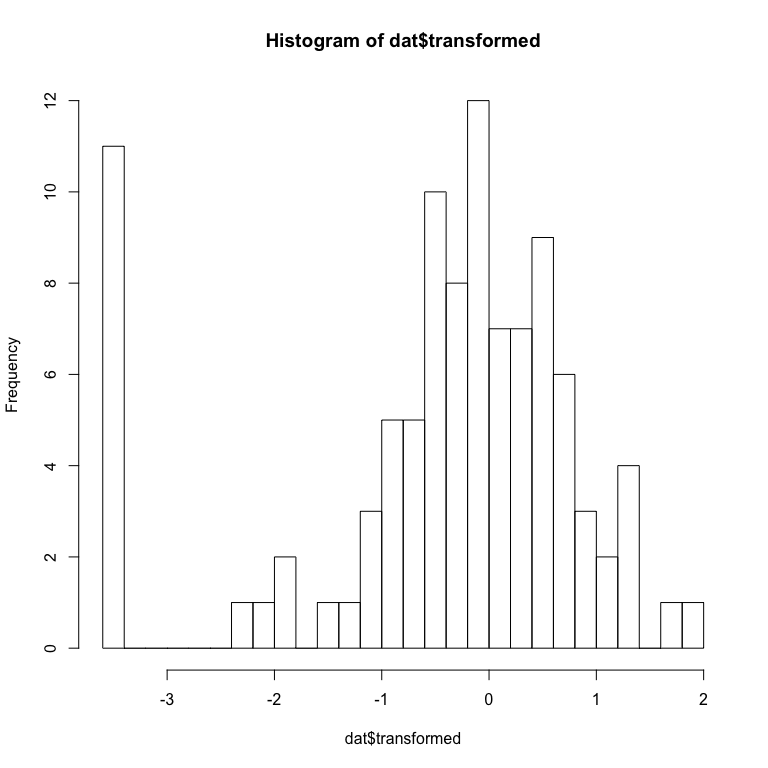
\includegraphics[width=\maxwidth]{figure/unnamed-chunk-5-1} \end{Schunk}
\caption{ein hypothetischer Datensatz aus vier Beobachtungen, die identische übliche Kennzahlen aufweisen, wie z.B. Mittelwert, Varianz, Korrelation, Regressionslinie, etc.}
\label{fig: Anscombes Quartet}
\end{center}
\end{figure}


\subsection{Grundsätze der Visualisierung}

Ein Grundsatz\marginnote{Beispiele für verzerrte Grafiken \href{https://en.wikipedia.org/wiki/Misleading_graph}{siehe}} von Grafiken und Darstellungen ist, die Daten so einsehbar und wahr wie möglich darzustellen. Der Leser sollte einen bestmöglichen überblick in kürzester Zeit über die Daten erhalten. Zusätzlich sollten die Graphen natürlich auch anschaulich sein. Vorab ein paar generelle Tipps, die vielleicht helfen könnten:

\begin{itemize}
\item Einfach ist besser, als kompliziert
\item Vermeide übertriebene Farben. Graphen sollten wenn möglich auch in schwarz-weiß leserlich sein (benutze einen Farbgradienten, der gleichzeitig ein Intensitätsgradient ist; benutze zusätzlich zu Farben auch gestrichelte Linien). Wenn dein Graph auf Farben basiert, achte darauf welche zu verwenden, die auch Menschen mit einer Rot-Grün-Schwäche erkennen können.
\item Ehrlichkeit: vermeide Verzerrungen. Benutze quadratische Formen, außer es gibt besondere Gründe. Achsen sollten bei 0 beginnen, außer es gibt gute Gründe, die dagegen sprechen. Verwende die gleiche Skala bei der Darstellung mehrerer Grafiken, wenn es keine Gründe gibt, die dagegen sprechen. 
\item Manipuliere deine Grafiken nicht!
\item Ausgabe in einem Vektor-Format (pdf, eps, svg)
\end{itemize}

\begin{figure}[htbp]
\begin{center}

\setkeys{Gin}{width=\textwidth}
\begin{Schunk}

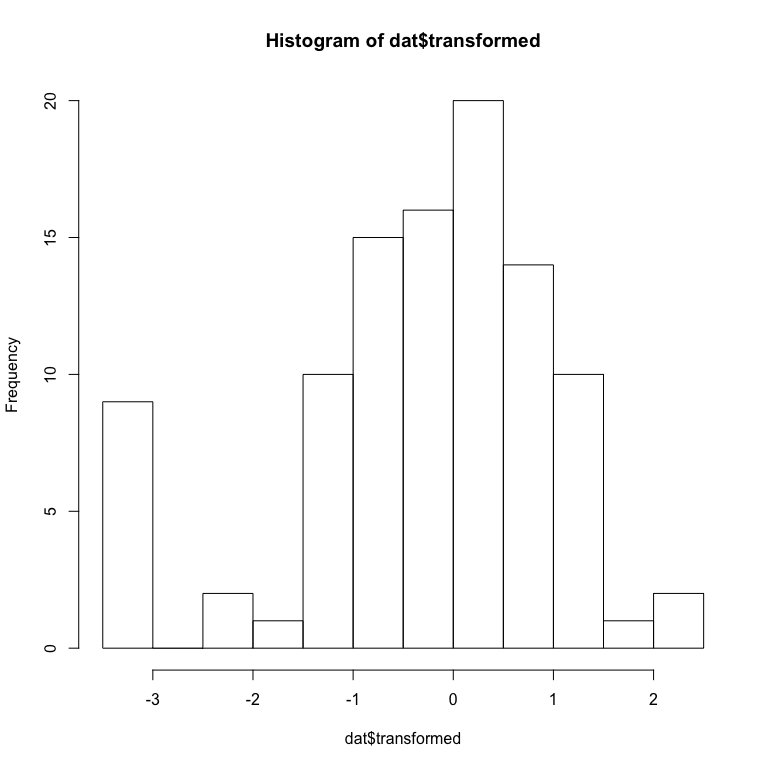
\includegraphics[width=\maxwidth]{figure/unnamed-chunk-6-1} \end{Schunk}
\caption{Vier typische Plot-Typen, von oben links nach unten rechts: a) Liniendiagramm, repräsentiert stetige Messungen einer Variablen; b) Streudiagramm, repräsentiert eine Beziehung zwischen zweier stetigen Variablen; c) Balkendiagramm, repräsentiert Messungen in unstetigen Gruppen / Variablen; d) Boxplot, repräsentiert stetige Messungen in unstetigen Gruppen.}
\label{fig: exaple plots}
\end{center}
\end{figure}


\subsection{Graphen-Typen}

Es gibt eine große, fast unendliche Bandbreite an verschiedenen visuellen Darstellungen von Datensätzen. Im Folgenden werden nun vier häufig verwendete Graph-Typen gezeigt. 

\paragraph{Liniendiagramme:} Liniendiagramme werden benutzt, um stetige, geordnete Messwerte darzustellen. Typische Beispiele hierfür wären Zeitreihen, stetige Parameterveränderungen oder mathematische Funktionen. Beispiel siehe Fig.~\ref{fig: exaple plots} a.

\paragraph{Streudiagramme:} Streudiagramme veranschaulichen zwei stetige Variablen die paarweise gemessen wurden. Ein typisches Beispiel hierfür wäre das wiederholte Messen von verschiedenen Variablen mit der Absicht herauszufinden, ob diese korrelieren. Beispiel siehe Fig.~\ref{fig: exaple plots} b.

\paragraph{Balkendiagramme:} Balkendiagramme beinhalten Informationen (Zählungen oder stetige Variablen) über unstetige Gruppen. Beispiel siehe Fig.~\ref{fig: exaple plots} c.

\paragraph{Boxplots:} Boxplots benutzt man häufig bei der Verteilung einer stetigen Variable über mehrere unstetige Gruppen. Klassischerweise bestehen sie aus einer Box, 'Whiskers' (Linien) und gegebenfalls Punktewerte um die 'Whiskers'. Deren Bedeutung ist von der benutzten Software abhängig, mit der man die Plots gestaltet hat. Normalerweise bedeckt die Box die in der Mitte liegenden 50\%, mit dem angedeuteten zentralen Medianwert. Die Linien sollen zur Abschätzung der Daten-Bandbreite dienen, Ausreißer ausgenommen. Natürlich liegt es im Auge des Betrachters, was als Ausreißer angesehen wird und was nicht. Die exakte Definition von Whiskers besagt, dass die weit entfernteste Beobachtung weniger oder gleich der oberen Quantile plus 1,5 der Länge der Interquartilenbreite ist. Beispiel siehe Fig.~\ref{fig: exaple plots} d.

\vspace{1cm}
\begin{fullwidth}
\begin{mdframed}
    
\textbf{In R:} 

Es gibt viele gute Einleitungen in Graphiken mit R, sodass diese Details hier nicht weiter aufgeführt werden. Zu Beginn empfehle ich diese  \href{https://github.com/florianhartig/ResearchSkills/tree/master/Labs/Statistics/Practicals/GraphicsInR}{übungen zum graphischen Gestalten mit R}. Diese sind begleitend zu diesem Skript, oder auch zu

\begin{itemize*}
  \item \href{http://www.statmethods.net/graphs/index.html}{QuickR}
  \item \href{http://shinyapps.org/apps/RGraphCompendium/index.php}{RGraphCompendium}
  \item \href{http://www.uni-kiel.de/psychologie/rexrepos/rerDiagrams.html}{rexrepos}
\end{itemize*}

\end{mdframed}
\end{fullwidth} 


\chapter{Inferenzstatistik}

\marginnote{Inferenzstatistik ist das Ziehen von Schlüssen aus Beobachtungen durch statistische Methoden} 

Inferenzstatistik behandelt das Schlussfolgern, z.B. das Rückschlüsse ziehen aus Beobachtungen. Ein Beispiel einer solchen Folgerung wäre beispielsweise die Beobachtung, dass 15 von 20 Testobjekte, die eine bestimmte Medikation erhielten (Behandlungsgruppe), eine Verbesserung ihres Zustandes zeigten --> Statistische Folge: Wir können davon ausgehen, dass es eine Wahrscheinlichkeit von X gibt, dass die Medikation einen positiven Effekt hat.


\section{Datenerzeugendes Modell}

\marginnote{Inferenzstatistik ist nicht immer, aber meist mit dem Prinzip des datenerzeugenden Modells verknüpft}

Eine zentrale Idee von vielen Methoden der Inferenzstatistik ist das Prinzip des datenerzeugenden Modells. Kurz gesagt beinhaltet unser datenerzeugendes Modell unsere festgelegte Annahme, wie die Daten entstehen (normalverteiltes Rauschen, lineare Reaktion). Daraus kann man dann abhängig unserer festgelegten Annahme die unbekannten Größen (Unterschiede zwischen Behandlungsgruppe und Kontrollgruppe) berechnen (schlussfolgern).

\marginnote{In der Statistik verwendet man oft das Wort "`behandelt"' um Veränderungen in experimentellen Einheiten zu beschreiben. Hier wären die zwei Musikarten "`Behandlung"' und das "`Nichts-tun"' die Kontrolle} 

Man stelle sich vor man möchte herausfinden, ob das Pflanzenwachstum von Musik beeinflusst werden kann. Hierzu nehmen wir zwei Töpfe, jeder mit einer Pflanze, wobei eine mit klassischer und eine andere mit Heavy Metal -Musik beschallt wird. Eine der beiden wird zwangsläufig höher wachsen, jedoch könnte dies reiner Zufall sein, da es immer Variationen in Wachstumsraten gibt.

Somit bedarf es mehrerer Wiederholungen. Nun nehmen wir im unten aufgeführten Beispiel 30 Töpfe.

\begin{figure}[htbp]
\begin{center}
\begin{Schunk}

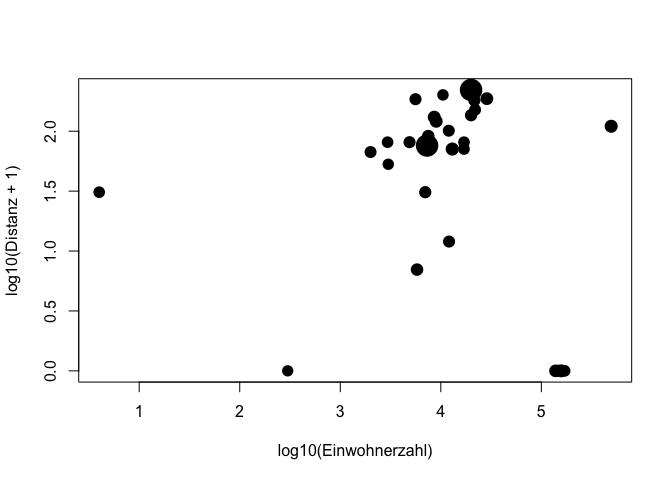
\includegraphics[width=\maxwidth]{figure/unnamed-chunk-7-1} \end{Schunk}
\caption{Wachstumsmessungen unter verschiedenen Behandlungsweisen}
\label{fig: plant growth music}
\end{center}
\end{figure}

\marginnote{Beachte die Interpretation eines Boxplots - die dickere Linie in der Mitte der Box ist der Medianwert. Die Box bedeckt die zentrale 0,5 Quantile der Verteilung}
Es scheint Unterschiede zwischen den drei Fällen zu geben, jedoch gab es auch Abweichungen in den Wachstumsraten innerhalb der einzelnen Behandlungsguppen (durchschnittlich haben wir hier sieben Beobachtungen pro Behandlung). Somit ist es immer noch möglich, dass die Unterschiede in den Beobachtungen durch Zufall entstanden sind.

Wenn wir genaue Aussagen über die Wahrscheinlichkeit der Unterschiede zwischen den zwei behandelten und der Kontrollgruppe treffen möchten, müssen wir ein Modell erstellen, welches die stochastische Abweichung in den Daten beschreibt. Dies erlaubt uns wiederum Eigenschaften, wie z.B. die Zufallswahrscheinlichkeit der beobachteten Unterschiede berechnen zu können. Diese Annahmen sind das, was wir als statistisches Modell bezeichnen (oder auch: stochastische Verfahren, datenerzeugendes Modell). 

Die üblichere Modellart für solche Zwecke ist das parametrische statistische Modell. Für die Daten, die wir hier haben, würde das parametrische statistische Modell annehmen, dass es eine durchschnittliche Wachstumsrate für jede Behandlungsart (Kontrolle, klassische und Heavy Metal Musik) gibt, jedoch das Wachstum jeder individuellen Pflanze mit einer normalverteilten Abweichung um ihre behandlungsspezifische durchschnittliche Wachstumsrate variiert. Die Parameter dieses Modells sind die unbekannten durchschnittlichen Wachstumsraten und die Abweichung der Normalverteilung. Diese Parameter werden dann mit Methoden, die hier in diesem Kapitel erklärt werden, an die Daten angepasst und basieren auf der Berechnung für z.B. die Wahrscheinlichkeit der Datenresultate, wenn keine Unterschiede zwischen den Gruppen wären.

Eine andere Möglichkeit, um datenerzeugende Modelle zu erstellen, sind nicht-parametrische Methoden.\marginnote{Die nicht-parametrische Statistik versucht Vermutungen über datenerzeugende Prozesse zu vermeiden. Normalerweise entsteht der datenerzeugende Prozess durch das Imitieren der eigentlichen Daten, z.B. durch das erneute Prüfen von Methoden.} Nicht-parametrische Methoden umgehen die Notwendigkeit einer Annahme z.B. über die Streuung der Daten durch das Randomisieren (zufälliges Anordnen) oder das wiederholte Prüfen des Datensatzes. Wie funktioniert das? Für das Pflanzenwachstum beispielsweise lässt sich diese Frage wie folgt beantworten: Wie wahrscheinlich wäre das erneute Erhalten der beobachteten Ergebnisse, wenn keine Unterschiede zwischen den Gruppen wären und ohne das Anstellen von Vermutungen über die Streuung? Hierfür werfen wir einfach alle Beobachtungen ungeachtet ihrer Behandlungsart in einen Topf und verteilt sie erneut zufällig in die drei Behandlungsgruppen. Wenn wir dies nun oft wiederholen (z.B. 1000 mal) kann man einen guten Eindruck davon bekommen, wie wahrscheinlich es ist die beobachteten Unterschiede zu erhalten, wenn die Behandlungen keinen Effekt hätten.

Nicht-parametrische Methoden sind ein wichtiger Bestandteil moderner Statistik.\marginnote{Die Feinsinnigkeit der parametrischen Methoden baut auf das Treffen von Annahmen, was in einer Art und Weise zusätzliche Daten darstellt. Natürlich basieren dann alle Ergebnisse auf der Richtigkeit dieser Vermutungen. Wie man parametrische Vermutungen überprüft werden wir später in diesem Kapitel behandeln.} Ihr Vorteil liegt wohl in der Tatsache, dass sie keine Vermutungen anstellen. Andererseits sind parametrische Methoden meist viel schneller und sind, falls ihre Annahmen korrekt sind, mit der selben Menge an Daten viel aussagekräftiger und feinfühliger, wodurch sie viel wahrscheinlicher einen Effekt, falls vorhanden, erkennen können. Aufgrund der letzten beiden Argumente sind momentan parametrische Methoden die Grundlage der meisten statistischen Analysen.


\section{Inferentielle Outputs}

Auf dem datenerzeugendem Modell basierend (parametrisch oder nicht-parametrisch) können wir nun verschiedene inferentielle Vorgehensweisen anwenden, um Rückschlüsse über unsere Daten (in unserem Fall: Um entscheiden zu können, ob Musik einen Unterschied macht, oder nicht) zu ziehen. In der üblichen Statistik gibt es vorwiegend zwei inferentielle Vorgehensweisen, die auf alle möglichen Arten von Konfigurationen und Modelle angewendet werden. Die Outputs dieser zwei Vorgehensweisen sind: p-Werte und Maximum-Likelihood-Schätzwerte. Ein weiteres drittes Verfahren wird momentan immer beliebter - die nachträglich, durch Bayes ermittelte Inferenz. Auf diese werde ich noch am Ende dieses Abschnittes eingehen.

\subsection{p-Werte}

Die Verwendung des p-Wertes ist eng mit der Inferenzmethode der Null-Hypothesen Signifikanzprüfung (null hypothesis significance testing, NHST) verbunden. Die Idee, die dahinter steckt, ist Folgende: wenn wir gewisse Daten beobachten und ein statistisches Modell haben, können wir dieses statistische Modell benutzen, um eine vorgegebene Hypothese über das Entstehen der Daten zu präzisieren. Für das Beispiel der Pflanzen und der Musik könnte unsere Hypothese so lauten: "`Musik hat keinen Einfluss auf Pflanzen; alle beobachteten Unterschiede basieren auf zufälligen Abweichungen zwischen den Individuen."' Dieses Szenario wird als Nullhypothese bezeichnet. \marginnote{Eine Nullhypothese $H_0$ ist ein vorgegebenes Szenario, das Vorhersagen über erwartete Wahrscheinlichkeiten von verschiedenen Beobachtungen macht.} Auch wenn es üblich ist, die Annahme keinerlei Auswirkungen auf die beobachteten Objekte als Nullhypothese zu setzen, ist es tatsächlich die eigene Entscheidung und man könnte genauso gut die Vermutung "`klassische Musik verdoppelt die Wachstumsrate der Pflanzen"' als Nullhypothese setzen. Es liegt im Ermessen des Analytikers, was als Nullhypothese betrachtet werden soll. Dies ist auch der Grund für die große Auswahlmöglichkeit an verfügbaren Tests. Wir werden noch einige davon im folgenden Kapitel über wichtige Hypothesentests kennen lernen.

Wenn wir uns für eine Nullhypothese entschieden haben, berechnen wir die Wahrscheinlichkeit für dieses oder ein extremeres Beobachten der Daten in diesem Szenario. \marginnote{Der p-Wert ist die Wahrscheinlichkeit die Daten oder extremere Daten unter unserer Nullhypothese beobachten zu können.} 

\begin{equation}
p := p(d >= D_{obs} | H_0)
\end{equation}

Wenn der p-Wert unter eine gewisse Schwelle sinkt (das sog. Signifikanzlevel $\alpha$), spricht man von einem signifikantem Beweis, um die Nullhypothese abzuweisen. Die Schwelle $\alpha$ ist eine Vereinbarung, in der ökologie üblicherweise 0.05, sodass ein p-Wert kleiner als 0.05 ein Abweisen der Nullhypothese veranlässt. \marginnote{Wenn p<0.05, haben wir signifikante Beweise für ein Abweisen der Nullhypothese.} 

Ein Problem der Hypothesentests und der p-Werte ist die notorische Fehlinterpretation der Ergebnisse. Der p-Wert ist NICHT die Wahrscheinlichkeit, dass die Nullhypothese wahr, oder die Alternativhypothese falsch ist; auch wenn viele Autoren diesen Fehler bei ihrer Interpretation gemacht haben, wie z.B. \citep[][]{Cohen-earthisround-1994}. Eher kann man den p-Wert als eine Kontrolle der Falsch-Positiven-Rate ansehen (Typ I-Fehler). Wenn man Hypothesentests mit einem $\alpha$ -Level von 0.05 auf Zufallsdaten anwendet, erhält man exakt 5\% Falsch-Positive. Nicht mehr und auch nicht weniger.  

\subsection{Maximum-Likelihood-Schätzwert}

Eine zweite Variante der Ergebnisdarstellung, welche bei den meisten statistischen Methoden verwendet wird, ist das Schätzen von Maximum-Likelihood Parametern. Zusammenfassend kann man sagen, dass die Maximum-Likelihood-Schätzung (maximum-likelihood estimate (MLE)) die beste Schätzung für Parameter in unserem Modell ist (z.B. Unterschiede zwischen den Behandlungsarten und der Kontrolle, wie in unserem Beispiel).


Genauer gesagt wird die Wahrscheinlichkeit in der Statistik als Funktion der Modellparameter $\theta$ beschrieben als

\begin{equation}
L(\theta) := p(dD_{obs} | M(\theta))
\end{equation}

, z.B. als die Funktion die man erhält, wenn man die Wahrscheinlichkeit der erhaltenen beobachteten Daten bei veränderten Modellparameter berechnet.

Der Maximum-Likelihood-Schätzwert\marginnote{Hier ist zu beachten, dass die Maximum-Likelihood-Schätzung ein Parametersatz ist, für den die Daten am Wahrscheinlichsten sind, nicht jedoch der wahrscheinlichste Parametersatz!} ist weiterhin definiert als eine Kombination von Parametern oder Modellannahmen, für welche die Wahrscheinlichkeit maximal ist. Während der p-Wert die Wahrscheinlichkeit der beobachteten 
oder extremeren Daten unter einer festgelegten (Null-) Hypothese beschreibt, gibt uns der Maximum-Likelihood-Schätzwert die "`Hypothese"' mit der höchsten Wahrscheinlichkeit an unsere beobachteten Daten zu erhalten.

Die Maximum-Likelihood-Schätzung ist nur ein einzelner Parameterwert.\marginnote{Eine Punktschätzung ist vergleichbar mit einer einzelnen besten Schätzung.} Diese Art Schätzung wird oft Punktschätzung genannt. Jedoch ist eine Punktschätzung oft unbrauchbar, wenn wir nicht wissen wie genau sie ist.\marginnote{Konfidenzintervalle bieten einen Unsicherheitsschätzwert um die Punktschätzung herum.} Deswegen werden Parameterschätzungen immer mit Konfidenzintervallen angegeben. Salopp kann man sagen, dass das 95\% Konfidenzintervall eines Parameters eine wahrscheinliche Reichweite für diesen Bereich ist. Verwirrend ist hier, dass dies nicht das Intervall ist, in dem der richtige Parameter mit 95\% Wahrscheinlichkeit liegt. Vielmehr beinhaltet das Standard 95\% Konfidenzintervall bei wiederholten Experimenten zu 95\% aller Fälle den richtigen Wert. Dies ist ein kleiner, aber entscheidender Unterschied. Jedoch machen wir uns hierüber nun keine weiteren Gedanken. Das Konfidenzintervall ist der ungefähre Bereich, in dem wir den korrekten Parameter erwarten. 

\vspace{1cm}
\begin{fullwidth}
%\begin{mdframed}
    
\textbf{Übungsfragen MLE:} 
\textbf{4.1} Wie ist die Likelihood der beobachteten Daten D für ein gegebenes Modell M mit Parameter x definiert?
\textbf{4.2} In einem Experiment wurde der Effekt von Stickstoff auf das Wachstum von Pflanzen getestet - der Likelihood ist maximal für eine Verdoppelung des Wachstums. Die Autoren schreiben: “Die Wahrscheinlichkeit die beobachteten Daten zu erhalten ist maximal wenn man annimmt dass Stickstoff das Wachstum von den beobachteten Pflanzen verdoppelt” - ist diese Aussage Korrekt?
\textbf{4.3} Weiter unten schreiben die Autoren: “Der wahrscheinlichste Wert für den Effekt von Stickstoff ist 2 (verdoppelung)” - ist diese Aussage korrekt?

%\end{mdframed}
\end{fullwidth}

\subsection{Bayes Verfahren}

Um unsere\marginnote{Bayes'sche Verfahren berechnen eine dritte Größe, die posteriore Wahrscheinlichkeit. Auch wenn man diese auf jedes Modell anwenden kann, benutzt man sie üblicherweise bei erweiterten statistischen Berechnungen.} übersicht der schlussfolgernden Methoden zu komplettieren, fehlt noch eine, die erwähnt werden sollte - Bayes'sche Methoden berechnen eine Größe, die sich die posteriore Parameterschätzung (posterior parameter estimate) nennt. Diese ist ähnlich, jedoch nicht identisch zu der vorherigen Parameterschätzung. Näheres ist hier nicht von Nöten, bei Bedarf und Interesse kann jedoch meine Seite weiterhelfen \citep{Gelman-BayesianDataAnalysis-2003} \href{http://florianhartig.github.io/LearningBayes/}{Learning Bayes}.

\subsection{Verschiedene Methoden != verschiedene Modelle}

Wir wissen nun, dass es drei verschiedene Größen gibt, die Statistiker typischerweise berechnen: p-Werte, Maximum-Likelihood und die Posteriori. Man kann bei gegebenen datenerzeugenden Prozessen immer jede einzelne davon berechnen.

Ich\marginnote{ANOVA , T-Tests und lineare Regression sind nur unterschiedliche Begutachtungen des selben Modells} formuliere diesen Punkt konkreter, da fälschlicherweise viele Menschen glauben sie benutzen unterschiedliche Modelle, wobei sie lediglich unterschiedliche Wege nutzen, um diese zu begutachten. Ein Beispiel hierfür sind ANOVA, T-Tests und die lineare Regression. Alle basieren auf ein und dem selben datenerzeugenden Prozess - einige festgelegte Auswirkungen zwischen Gruppen und obendrein ein unabhängiger und identischer normalverteilter Fehler. ANOVA und T-Tests legen verschiedenste Nullhypothesen fest und die lineare Regression sucht nach dem Maximum-Likelihood-Schätzwert. Hier könnte man bei Bedarf noch die Bayes'sche Posteriori berechnen. 

\section{Wichtige Hypothesentests}

Nachdem jetzt die grundlegenden statistischen Datenausgaben besprochen wurden, gehen wir nun in die Praxis über, um die zwei wohl häufigsten Hypothesentests kennen zu lernen - den T-Test und ANOVA. Wie bereits erwähnt, basieren sie beide auf dem selben datenerzeugenden Prozess, legen jedoch geringfügig unterschiedliche Nullhypothesen fest.

\subsection{T-Test}

Ein T-Test testet die Unterschiede der Mittelwerte von zwei normalverteilten Stichproben; oder im Falle einer einzigen Stichprobe zwischen 0 und den Mittelwert der Stichprobe.\marginnote{Um bei unserer vorhergehenden Einteilung zu bleiben, würden wir unsere Response-Variable als stetig und den Prädiktor als kategorisch bezeichnen (Gruppe 1 oder Gruppe 2); oder im Falle einer einzelnen Gruppe gibt es keinen Prädiktor.} Erneut ist hier das zugrundelegende Modell das einer Normalverteilung mit der Nullhypothese, dass es keine Unterschiede zwischen den Mittelwerten der zwei normalverteilten Gruppen gibt, bzw. dass der Stichproben Mittelwert 0 ist, wenn wir nur eine Gruppe betrachten. Desweiteren sind Software-abhängig oft eine Reihe an Anpassungen möglich, z.B. eine Lockerung der Annahme, dass die zwei Gruppen die selbe Varianz aufweisen. Hier folgt nun ein Beispiel in R, mit klassischen Daten von \citet{Student-probableerrormean-1908}. Die Daten zeigen die Wirkung von zwei Schlafmitteln (gesteigerte Anzahl an Schlafstunden verglichen mit der Kontrolle) an 10 Patienten. 

\begin{figure}[htbp]
\begin{center}
\begin{Schunk}

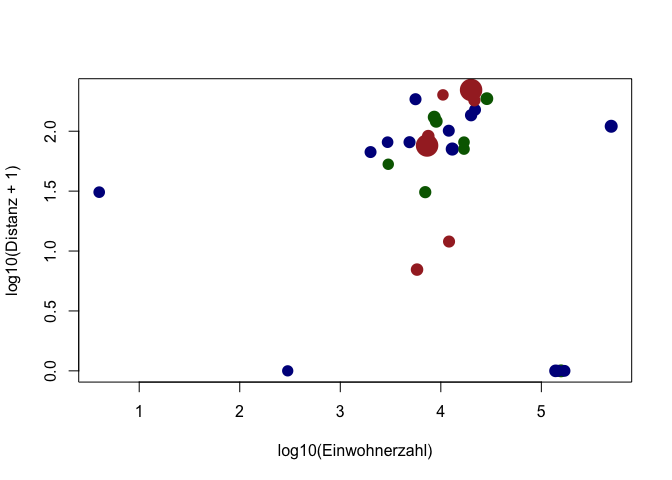
\includegraphics[width=\maxwidth]{figure/unnamed-chunk-8-1} \end{Schunk}
\caption{Daten von \citet{Student-probableerrormean-1908}}
\label{fig: Student Sleep Data}
\end{center}
\end{figure}

\begin{Schunk}
\begin{Sinput}
## Traditional interface
with(sleep, t.test(sleep$extra[sleep$group == 1], extra[group == 2]))
\end{Sinput}
\end{Schunk}

\begin{Schunk}
\begin{Sinput}
## Formula interface
t.test(extra ~ group, data = sleep)
\end{Sinput}
\begin{Soutput}

	Welch Two Sample t-test

data:  extra by group
t = -1.8608, df = 17.776, p-value = 0.07939
alternative hypothesis: true difference in means is not equal to 0
95 percent confidence interval:
 -3.3654832  0.2054832
sample estimates:
mean in group 1 mean in group 2 
           0.75            2.33 
\end{Soutput}
\end{Schunk}

Beachte, dass die Datenausgabe einen p-Wert (H0 = kein Unterschied), aber auch einen Maximum-Likelihood-Schätzwert der Mittelwertsvergleiche, zusammen mit den Konfidenzintervallen bietet. Dies geht weit über den klassischen T-Test hinaus. Vermutlich nahmen die Programmierer an, dass man zusätzlich den besten Schätzwert für die Mittelwertsunterschiede haben möchte.

Vorschlag für das Anzeigen des Ergebnisses: p>0.05: Unterschiede zwischen den Gruppen waren nicht signifikant. p<0.05: Wir erhielten einen Unterschied von X +- Konfidenzintervall zwischen den Gruppen (p-Wert für die Unterschiede eines T-Tests mit X). 

\vspace{1cm}
\begin{fullwidth}
%\begin{mdframed}
    
\textbf{Übungsfragen Hypothesentests:} 
\textbf{4.4} Definieren Sie den p-Wert.
\textbf{4.5} Wie ist in der vorherigen Definition “extremer” (also >=) definiert?
\textbf{4.6} Stellen Sie sich vor Sie leben in Venedig, und es gibt 3 Taxibootfirmen. Sie wollen wissen ob es Unterschiede in der Beförderungsgeschwindigkeit gibt und machen deshalb 300 Fahrten mit jeder Firma und stoppen die Zeit. Was wäre eine geignete Nullhypothese H0, um auf einen Unterschied zu testen?
\textbf{4.7} Bonusfrage: Nennen Sie eine der vielen möglichen sinnvollen Teststatistiken
\textbf{4.8} In der Physik gibt es das sogenannte Standardmodell, dass die Eigenschaften und Interaktionen der Material beschreibt. In den letzten 20 Jahren wurde das Standardmodell immer und immer wieder getestet, so “erfolgreich” dass die Physiker schon ein bisschen deprimiert sind weil Sie nichts neues entdecken. Was ist die Nullhypothese die bei diesen Tests angewandt wird?
\textbf{4.9} Sie lesen einen Artikel über ein medizinisches Experiment. Getestet wurde ein Medikament gegen eine Kontrolle, und der p-Wert ist 0.03. Die Studie schreibt: “Die Wahrscheinlichkeit dass das Medikament nicht wirkt ist 3\%” - stimmen Sie zu?
\textbf{4.10} Schreiben Sie eine korrekte Interpretation des obigen Ergebnis auf.
\textbf{4.11} Definierent Sie den Typ I Fehler (falschen positive).
\textbf{4.12} Wie viel Typ I Fehler erwarten Sie bei einen Signifikanzlevel von 7\%?
\textbf{4.13} Definieren Sie den Typ II Fehler (falsche negative).
\textbf{4.14} Wie viel Typ II Fehler erwarten Sie bei einen Signifikanzlevel von 7\%?
\textbf{4.15} Nennen Sie 2 Faktoren die Typ II Fehler beeinflussen, und die Richtung des Einflusses (negativ = Typ II nimmt ab wenn Faktor hoch geht).
\textbf{4.16} Definieren Sie die Teststärke / Power.
\textbf{4.17} Sie testen 100 Gene auf eine Assoziation mit Krebs. Bei 5 Genen zeigt der Test Signifikanz an. Wie bewerten Sie dieses Ergebnis?
\textbf{4.18} Sie bekommen von einer allwissenden Macht die Zusatzinformation dass Sie in dem oben genannten Test eine Teststärke von 99\% hatte. Sind Sie nun zuversichtlicher dass Sie einen Effekt gefunden haben?
\textbf{4.19} Definieren Sie die False Discovery Rate (FDR).
\textbf{4.20} Wovon hängt die FDR ab?
\textbf{4.21}  In einer Reihe von Experimenten testen Sie Medikamente auf eine Wirkung. Ihre Power ist 100\%. Sie schätzen dass jedes 20. Medikament das Sie testen eine Wirkung haben solte. Wie ist ihre FDR bei einem Signifikanzlevel von 5\%? Es reicht wenn Sie den Rechenweg aufschreiben, Sie müssen den Wert nicht ausrechnen.

%\end{mdframed}
\end{fullwidth}


\subsection{Varianzanalyse (ANOVA)}

ANOVA (analysis of variance) oder Varianzanalyse kann von verschiedenen Personen unterschiedlich verstanden werden. Die Standard-ANOVA macht grundsätzlich die gleichen Annahmen wie ein T-Test (normalverteilte Resonanz), jedoch für mehr als zwei Gruppen. Genauer gesagt testet es, ob die gemessene Response (z.B. eine abhängige Variable) von einem oder mehreren kategorischen Variablen mit zwei oder mehreren interagierenden Ebenen beeinflusst wird. Eine Wechselwirkung\marginnote{Eine Wechselwirkung: eine Variable verändert die Auswirkung einer anderen Variablen} zwischen zweier Variablen bedeutet, dass sich der Wert einer erläuternden Variable darauf auswirkt, wie sehr eine andere erläuternde Variable die Response beeinträchtigt.

Während der Begriff ANOVA meist mit der oben genannten Erklärung in Verbindung gebracht wird (welche der von T-Tests / linearer Regression entspricht, siehe nächstes Kapitel), kann die Auffassung der ANOVA in der gleichen Weise erweitert werden, wie ein lineares Regressionsmodell zu einem allgemeinen linearen Modell (engl. Generalized Linear Models, glm) erweitert werden kann etc. Dies erlaubt uns also, ANOVAs auf Modelle mit nicht-normalverteilten Fehlern anzuwenden (natürlich muss dies der Software gesagt werden, es geht nicht automatisch davon aus). Deswegen muss man besonders Acht darauf geben, von was andere ausgehen, wenn sie diesen Term benutzen.

Hier ist ein einfaches Beispiel mit einer Standard-ANOVA (normalverteilte Fehler), in der getestet werden soll, ob Gewicht (von Hühnern) von ihrer Ernährung abhängt, wobei 'Ernährung' ein variabler Faktor mit vier Stufen ist:

\begin{Schunk}
\begin{Sinput}
aovresult <- aov(weight~Diet, ChickWeight)
summary(aovresult)
\end{Sinput}
\begin{Soutput}
             Df  Sum Sq Mean Sq F value   Pr(>F)    
Diet          3  155863   51954   10.81 6.43e-07 ***
Residuals   574 2758693    4806                     
---
Signif. codes:  0 '***' 0.001 '**' 0.01 '*' 0.05 '.' 0.1 ' ' 1
\end{Soutput}
\end{Schunk}

Wir erhalten einen p-Wert von 6.43e-07, welcher mit einem $\alpha$ Level von 0.05 höchst signifikant ist. Somit können wir die Nullhypothese abweisen, dass die Ernährung keinen Einfluss auf die Response "`Gewicht"' habe. Beachte hier, dass wir keine Parameterschätzwerte erhalten und wir keine Aussagen darüber machen können, welche Ernährung sich von welcher unterscheidet. Hierfür gibt es zwei Möglichkeiten:

\begin{itemize}
\item Entweder wendet man den sogenannten Post-Hoc-Test an, welcher auf Unterschiede der Ernährungsweisen testet (Bsp. mit einem T-Test).
\item Oder man wechselt zu einer Regression, die im folgenden Kapitel genauer beschrieben wird.
\end{itemize}

Mit einem Post-Hoc-Test wendet man multiple Tests auf die gleichen Daten an. Dies kann zum Problem werden - der Grundgedanke des p-Werts ist eine Wahrscheinlichkeitkalkulation für das Betrachtet der Daten bezüglich EINER Nullhypothese. Nach einer solchen Durchführung erhält mal allenfalls einen  5\% Fehler bei einem $\alpha$ Level von 0.05. \marginnote{Beim Anwenden multipler Tests auf die selben Daten benötigt man eine Korrektur des p-Werts für multiples Testen.} Wenn wir jedoch multiple Tests durchführen, testen wir auch multiple Nullhypothesen und es ergeben sich mehr Möglichkeiten für die Testgrößen ein Signifikanzlevel nur durch Zufall zu erreichen. Deswegen müssen wir den p-Wert für multiples Testen korrigieren. Um hierzu mehr Informationen zu erhalten, ist Google dein bester Freund. 

\subsection{Weitere wichtige Tests}

T-Tests und ANOVA sind sehr häufig verwendete Tests, wobei es noch viele weitere gibt. Eine Liste mit Tests kann man beispielsweise im Wikipedia-Artikel unter diesem \href{http://en.wikipedia.org/wiki/Category:Statistical_tests}{Link} finden.


\section{Regression}

Wie schon zuvor beschrieben, bedeutet Regression nicht zwingend, dass man ein anderes statistisches Modell wie bei Hypothesentests verwendet (ANOVA und das lineare Regressionsmodell verwenden in R die gleichen Annahmen). Nichtsdestotrotz ist das Ziel einer Regression ein anderes. Während Hypothesentests nur überprüfen, ob die Daten mit einer Nullhypothese vereinbar sind, sucht eine Regression nach einer am besten passenden Hypothese oder Parametern (Maximum-Likelihood-Schätzwert). Somit sucht ein Regressionsmodell nach einer Parameterkombination, die mit der höchsten Wahrscheinlichkeit die beobachteten Daten, mit vorgegebenen Modellannahmen, ausgibt.

\subsection{Lineare Regression}

Das grundlegendste Regressionsmodell ist die lineare Regression. Hier lautet die Annahme, dass wir eine Response haben, die von einem Prädiktor wie folgt abhängt:

\begin{equation} \label{eq: linear regression}
y \sim a \cdot x + b + \epsilon 
\end{equation}

wobei y die Response, x der Prädiktor ist; a ist der Parameter, wie sehr der Prädiktor die Response beeinflusst, b ist der Schnittpunkt und $\epsilon$ ist die Zufallsvariation, welche in einer linearen Regression als normalverteilt angenommen wird.

In R wird solch eine Regression durch folgenden Befehl erreicht

\begin{Schunk}
\begin{Sinput}
fit = lm(airquality$Temp~airquality$Ozone)
summary(fit)
\end{Sinput}
\begin{Soutput}

Call:
lm(formula = airquality$Temp ~ airquality$Ozone)

Residuals:
    Min      1Q  Median      3Q     Max 
-22.147  -4.858   1.828   4.342  12.328 

Coefficients:
                 Estimate Std. Error t value Pr(>|t|)    
(Intercept)      69.41072    1.02971   67.41   <2e-16 ***
airquality$Ozone  0.20081    0.01928   10.42   <2e-16 ***
---
Signif. codes:  0 '***' 0.001 '**' 0.01 '*' 0.05 '.' 0.1 ' ' 1

Residual standard error: 6.819 on 114 degrees of freedom
  (37 observations deleted due to missingness)
Multiple R-squared:  0.4877,	Adjusted R-squared:  0.4832 
F-statistic: 108.5 on 1 and 114 DF,  p-value: < 2.2e-16
\end{Soutput}
\end{Schunk}

\begin{figure}[htbp]
\begin{center}
\begin{Schunk}

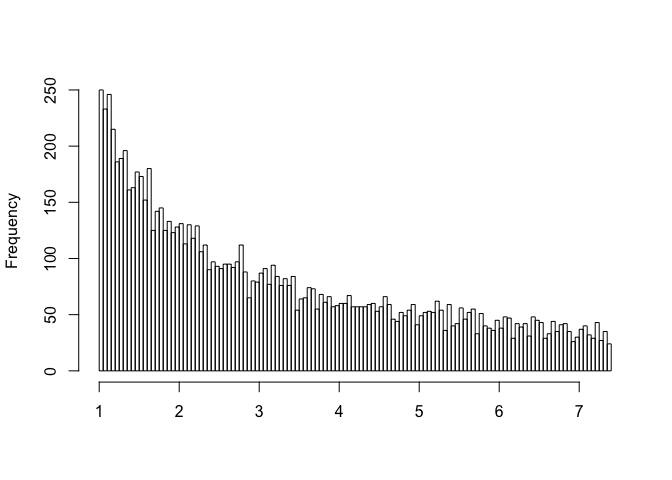
\includegraphics[width=\maxwidth]{figure/unnamed-chunk-13-1} \end{Schunk}
\caption{Luftqualitäts Datensatz: Temperatur aufgetragen gegen Ozon. Zusammenhang durch die Regressionsgerade angegeben.}
\label{fig: LR}
\end{center}
\end{figure}

Dieser Code kann unabhängig davon verwendet werden, ob der Prädiktor stetig oder kategorisch ist. Im Falle einer stetigen Variable entsteht eine Linie anhand der Daten. Im Falle einer kategorischen Variable mit n Stufen ist die erste Stufe als Referenz gesetzt (Schnittpunkt), und n-1 Faktoren entsprechen den folgenden Stufen, die den Unterschied zur Referenz beschreiben.

Die entsprechenden Parameter erscheinen in der Spalte "`Estimate"'. Dies zeigt uns, wie sehr der Prädiktor, in diesem Fall Ozon, die Response, hier Temperatur, beeinflusst: Für jede Einheit Ozon mehr steigt die Temperatur um 0.201 Einheiten, mit einem Standardfehler (Konfidenzintervall) von 0.019. Abgesehen davon, wie ein Regressions-Output aussieht, lehrt uns dies etwas anderes Wichtiges: Die Tatsache, dass wir die Temperatur als Response und Ozon als Prädiktor benutzt haben, bedeutet nicht, dass Ozon ursächlich die Temperatur beeinflusst. \marginnote{Korrelation ist nicht Kausalität.}Tatsächlich ist es genau anders herum: wenn wir mehr Sonne haben, wird es wärmer und wir haben tendenziell mehr Ozon. Regression schafft nicht, wie die meisten anderen statistischen Analysen, Kausalität. Es schafft Korrelation. Was wir hier ausdrücken ist, dass wenn unsere Ozonmessungen steigen, wir ziemlich sicher davon ausgehen können, dass es auch gleichzeitig wärmer wird. Was wiederum nicht bedeutet, dass Ozon Hitze erschafft. Korrelation ist nicht Kausalität.

Die Regressionsergebnisse geben uns ebenfalls einige p-Werte aus. Das sind die Ergebnisse von mehreren Hypothesentests, die automatisch nach der Regression geschaltet sind. Beispielsweise erhält man einen p-Wert für jeden Parameter. Dieser p-Wert basiert auf einem bestimmten Typ von T-Test, wobei das vollständige Modell gegen ein Modell mit auf 0 gesetzten Parametern getestet wird. Zusätzlich gibt es noch einen weiteren p-Wert, welcher auf einer anderen Testgröße am Ende der Regressionsausgabe beruht. Dieser testet die Nullhypothese mit allen Parametern gleich 0.

\vspace{1cm}
\begin{fullwidth}
\begin{mdframed}
    
\textbf{Präzisieren von verschiedenen Modellannahmen in R:} 

Response y hängt linear von Variable a (stetig oder kategorisch) ab

\begin{Schunk}
\begin{Sinput}
fit = lm(y~a)
summary(fit)
\end{Sinput}
\end{Schunk}

Response y hängt linear von zwei Variablen a und b (stetig oder kategorisch) ab, aber der Wert beider Variablen beeinflusst nicht den Effekt, welcher die andere Variable auf die Response hat (keine Interaktion)

\begin{Schunk}
\begin{Sinput}
fit = lm(y~a+b)
summary(fit)
\end{Sinput}
\end{Schunk}

Response y hängt linear von zwei Variablen a und b (stetig oder kategorisch) ab, aber der Wert der einen Variable beeinflusst nicht den Effekt der anderen Variable auf die Response (Interaktion)

\begin{Schunk}
\begin{Sinput}
fit = lm(y~a*b)
summary(fit)
\end{Sinput}
\end{Schunk}

Response y ist von einer Variablen a (stetig oder kategorisch) wie in $a + a^2$ abhängig

\begin{Schunk}
\begin{Sinput}
fit = lm(y~a + I(a^2))
summary(fit)
\end{Sinput}
\end{Schunk}

die Schreibweise I() kennzeichnet eine darauf folgende mathematische Formel. 

\end{mdframed}
\end{fullwidth}



\subsection{überprüfen der Annahmen}

Formal gesehen kann man jegliche Datensätze auf lineare Modelle übertragen. Jedoch sind hier wie bei jeder statistischen Folgerung die Ergebnisse (z.B. Parameterschätzungen, p-Werte) von den getroffenen Annahmen abhängig. Dementsprechend ist der p-Wert, den wir erhalten, von der Annahme abhängig, dass die Daten auch tatsächlich mit der Formel ~\ref{eq: linear regression} übereinstimmen. Wenn dies nicht der Fall ist, könnte der p-Wert völlig falsch sein. Somit muss man prüfen, ob diese Annahmen auch tatsächlich erfüllt wurden.

Also was genau waren die Annahmen einer linearen Regression? Ein Problem ist, dass sich Studenten an die Annahme der Normalverteilung erinnern. Deswegen überprüfen sie, ob die Response-Variable normalverteilt ist. Wenn man jedoch die Formel ~\ref{eq: linear regression} genauer betrachtet, erkennt man, dass dies nicht entscheidend ist. Wenn man die Terme in der Formel ~\ref{eq: linear regression} verschiebt,
sehen wir das, was eigentlich normalverteilt sein soll

\begin{equation} \label{eq: linear regression}
y - (a \cdot x + b ) \sim \epsilon 
\end{equation}

nämlich der Unterschied zwischen beobachtetem Wert und den Modellvorhersagen. Diese Unterschiede werden Residuen genannt und sollten, entsprechend unserer Modellannahmen, normalverteilt sein. Um zu überprüfen, ob dies wirklich der Fall ist, sollten einige Tests durchgeführt werden. Der einfachste Test ist das Erstellen eines Plots mit den Residuen gegen die angepassten Werte UND gegen alle Prädiktoren im Modell. Der daraus entstehende Plot erlaubt es dann viele mögliche Probleme zu erkennen (Fig.~\ref{fig: ResidualPatterns})

\begin{figure}[htbp]
\begin{center}
\begin{Schunk}

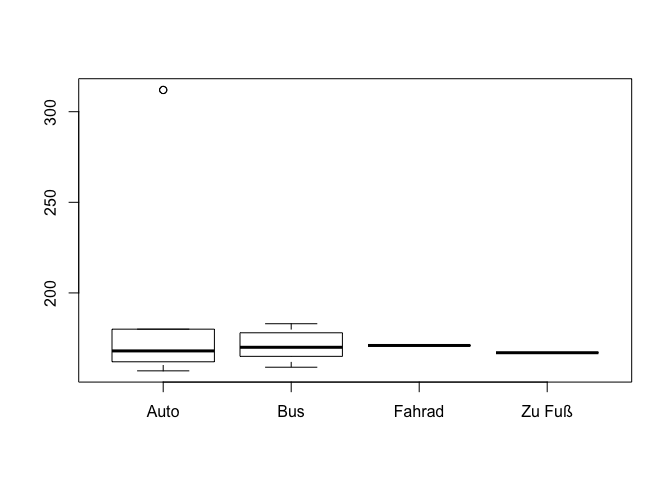
\includegraphics[width=\maxwidth]{figure/unnamed-chunk-18-1} \end{Schunk}
\caption{Eine Sammlung möglicher Muster, wenn die Residuen gegen den angepassten Wert (voreingestellt in R) oder einen Prädiktor geplottet werden.}
\label{fig: ResidualPatterns}
\end{center}
\end{figure}

übliche Probleme und ihre Lösungen sind  

\begin{itemize}
  \item Heteroskedastizität (Varianzveränderungen) --> Verändere die Response, oder verwende ein Regressionsmodell, das Heteroskedastizität berücksichtigen kann
  \item Muster in den Residuen -> Falsche Funktionsform des Regressionsmodells. Versuche Prädiktoren, quadratische Effekte, Interaktionen oder andere Dinge hinzuzufügen, die die funktionale Form ändern
  \item Verteilung nicht normal -> Angenommen, es liegt nicht an einem der früheren Probleme (kein Muster / keine Heteroskedastizität), kann man noch eine Variablentransformation ausprobieren oder eine Regression mit einer anderen Verteilungsannahme durchführen (siehe nächsten Abschnitt)
\end{itemize}  

Es gibt weitere spezialisierte Plots, um mit der Diagnose dieser Probleme zu helfen. Diese erfolgen bei der Anwendung des Befehls plot()


Sie erhalten grundlegende Residuendiagnosen durch Eingabe von plot(fit), wobei fit das angepasste Modell ist. Weitere Details zur Residuendiagnose siehe \href{http://www.statmethods.net/stats/rdiagnostics.html}{hier}.



\section{Allgemeine lineare Regressionsmodelle (GLM)}

Die allgemeine Vorstellung einer linearen Regression war, dass 1) die Response stetig ist, theoretisch von - unendlich bis + unendlich, und 2) Residuen normal um die Modellvorhersagen verteilt sind. Der Grundgedanke der allgemeinen linearen Regressionsmodell-Rahmenbedingung ist, wie zuvor in dem linearen Regressionsbeispiel zu arbeiten, jedoch beide Annahmen über Responsegrößen von - bis + unendlich und die Normalität zu lockern. Dazu müssen wir zwei Dinge tun

\begin{itemize}
  \item Um die Ausgabewerte in dem Bereich zu erhalten, den wir wollen, wickeln wir das lineare Modell in eine Transformationsfunktion, die die Response ins rechte Intervall zwingt (typische Intervalle sind positiv oder zwischen 0 und 1). Diese Transformation wird als Link-Funktion bezeichnet
  \item Um andere Verteilungen anzupassen, müssen wir dem Modell sagen, dass es etwas anderes als die Gaußsche Fehlerfunktion verwenden soll.
\end{itemize}    
   
Wir werden über diese Punkte nun etwas mehr ins Detail gehen.

\subsection{Die Link-Funktion}

Wir haben gesagt, dass eine lineare Regression folgende Form annimmt

\begin{equation}
y \sim a \cdot x + b 
\end{equation}

Das heißt, wenn x groß wird, könnte y jeden Wert einnehmen, positiv oder negativ. Ein Trick, um sicherzustellen, dass alle Vorhersagen für y positiv sind oder innerhalb eines bestimmten Bereichs liegen, ist eine Link-Funktion der Form

\begin{equation}
y \sim f^{link}(a \cdot x + b )
\end{equation}

Jede Funktion ist möglich, aber wie wir später sehen werden, sind typische Alternativen die Exponentialfunktion, die positive Ergebnisse garantiert, und die inverse Logit, die Bereich zwischen 0 und 1 garantiert.

\subsection{Andere Verteilungen}

Nun, das ist konzeptionell der einfache Teil, aber vielleicht ist noch nicht klar, welche Art von Distributionen neben der normalen vorhanden sind. Zwei typische Entscheidungen, die wir unten verwenden, sind die Binomial- (die Verteilung für das Münzwerfen) und die Poisson-Verteilung (eine diskrete Wahrscheinlichkeitsverteilung). Es stehen viele andere Möglichkeiten zur Verfügung. Vielleicht wird es deutlicher, wenn wir uns in den nächsten Abschnitten zu den konkreten Beispielen bewegen.

\subsection{0/1 Daten - logistische Regression}

Logistische Regression ist die häufigste Analyse für binäre Daten (Präsenz / Abwesenheit, überlebt / tot, infiziert / nicht infiziert). Logistische Regression geht davon aus, dass die Verteilung binomial ist (Münzwurf-Modell). Um den linearen Prädiktor auf einer Skala zwischen 0 und 1 zu erhalten, die für die Binomialverteilung erforderlich ist, verwenden wir die logistische Linkfunktion (oder inverse Logit).

\vspace{1cm}
\begin{fullwidth}
\begin{mdframed}
    
\textbf{In R:} 

Hier ein Beispiel mit den Daten der Titanik-überlebenden. Beachte, dass die Logit-Link automatisch ausgewählt wird, wenn in R die Binomialverteilung verwendet wird. Bei Bedarf könnte man diese Wahl überschreiben.

\begin{Schunk}
\begin{Sinput}
library(effects)
\end{Sinput}
\begin{Soutput}
Warning: package 'effects' was built under R version 3.3.2
\end{Soutput}
\begin{Sinput}
fmt <- glm(survived ~ age + I(age^2) + I(age^3), family=binomial, data = TitanicSurvival)
summary(fmt)
\end{Sinput}
\begin{Soutput}

Call:
glm(formula = survived ~ age + I(age^2) + I(age^3), family = binomial, 
    data = TitanicSurvival)

Deviance Residuals: 
    Min       1Q   Median       3Q      Max  
-1.5062  -0.9978  -0.9695   1.3483   2.0135  

Coefficients:
              Estimate Std. Error z value Pr(>|z|)    
(Intercept)  7.855e-01  3.031e-01   2.592 0.009549 ** 
age         -1.189e-01  3.291e-02  -3.613 0.000303 ***
I(age^2)     3.414e-03  1.113e-03   3.066 0.002171 ** 
I(age^3)    -2.931e-05  1.107e-05  -2.648 0.008109 ** 
---
Signif. codes:  0 '***' 0.001 '**' 0.01 '*' 0.05 '.' 0.1 ' ' 1

(Dispersion parameter for binomial family taken to be 1)

    Null deviance: 1414.6  on 1045  degrees of freedom
Residual deviance: 1398.5  on 1042  degrees of freedom
  (263 observations deleted due to missingness)
AIC: 1406.5

Number of Fisher Scoring iterations: 4
\end{Soutput}
\end{Schunk}


\end{mdframed}
\end{fullwidth} 




\subsection{Zähldaten - Poisson-Regression}

Die Poisson-Regression ist die Standard-Wahl für die Arbeit mit Zähldaten, obwohl ein paar andere Optionen zur Verfügung stehen. In der Poisson-Regression wird standardisiert eine Exponentialfunktion gewählt, um alle Werte positiv zu machen. Das Inverse des Exponentials ist der Log, also nennen wir das den Log-Link. Nach wie vor wählt R diese automatisch aus, wenn man angibt die Verteilung zu "`poissonieren"'.

\vspace{1cm}
\begin{fullwidth}
\begin{mdframed}
    
\textbf{In R:} 

Ein Beispiel hierfür zeigt einige Daten über die Fütterung von Nesthockern in Bezug auf ihre Attraktivität:
\begin{Schunk}
\begin{Sinput}
schnaepper <- read.csv(ßchnaepper.txt", sep="")
fm <- glm(stuecke ~ attrakt, family=poisson, data = schnaepper)
summary(fm)
\end{Sinput}
\begin{Soutput}

Call:
glm(formula = stuecke ~ attrakt, family = poisson, data = schnaepper)

Deviance Residuals: 
     Min        1Q    Median        3Q       Max  
-1.55377  -0.72834   0.03699   0.59093   1.54584  

Coefficients:
            Estimate Std. Error z value Pr(>|z|)    
(Intercept)  1.47459    0.19443   7.584 3.34e-14 ***
attrakt      0.14794    0.05437   2.721  0.00651 ** 
---
Signif. codes:  0 '***' 0.001 '**' 0.01 '*' 0.05 '.' 0.1 ' ' 1

(Dispersion parameter for poisson family taken to be 1)

    Null deviance: 25.829  on 24  degrees of freedom
Residual deviance: 18.320  on 23  degrees of freedom
AIC: 115.42

Number of Fisher Scoring iterations: 4
\end{Soutput}
\end{Schunk}

\end{mdframed}
\end{fullwidth} 


\subsection{Residuen-überprüfungen in allgemeinen linearen Regressionsmodellen}

Residuen in allgemeinen linearen Regressionsmodellen sollten nicht normalverteilt sein, deswegen verwendet man keine Standard-Kontrollen für Normalität wie normale Quantile-Quantile-Plots, um auf die Angemessenheit der Residuen zu überprüfen. Für nicht zu komplizierte Modelle gibt es eine Möglichkeit dieses Problem zu umgehen, indem man die sogenannten Pearsons-Residuen verwendet, die die beobachteten Unterschiede zwischen Modell und Daten durch die erwartete Varianz des Modells normiert \footnote{In R kann man die Option Pearson in vielen Funktionen angeben, einschließlich der Residual()-Funktion, die man auf ein angepasstes Objekt anwenden kann}

Ein Standardproblem in Poisson oder binomialen allgemeinen linearen Regressionsmodellen ist, dass die Varianz der Poisson- und Binomialverteilung nicht eingestellt werden kann, sondern durch den Mittelwert festgelegt wird. Dies ist ein Problem, das im normalen linearen Modell nicht auftritt, da hier der zufällige Teil durch eine Normalverteilung modelliert wird, die einen Parameter für die Varianz aufweist. Ein Problem, das sehr häufig in Poisson oder binomialen allgemeinen linearen Regressionsmodellen auftritt, ist eine überdispersion, d.h. dass die Residuen mehr Varianz, als unter dem angepassten Modell erwartet, zeigen. \marginnote{Man kann auf überdispersion prüfen, indem man die angepasste Abweichung betrachtet oder einen überdispersionstest anwendet} Der einfachste Weg, um dies zu korrigieren, ist die Verwendung der Quasi-Poisson- und Quasibinomialmodelle, die in der allgemeinen linearen Regressionsmodell-Funktion verfügbar sind. Diese Modelle bringen einen zusätzlichen Parameter ein, der die Varianz des Poisson- und des binomialen allgemeinen linearen Regressionsmodells abwandelt.

\vspace{1cm}
\begin{fullwidth}
%\begin{mdframed}
    
\textbf{Übungsfragen Regression:} 
\textbf{4.22} Was sind die Annahmen der linearen Regression?
\textbf{4.23} Wie werden die Parameter in der linearen Regression bestimmt?
\textbf{4.24} Welche H0 steckt hinter den p-Werten der Parameter der linearen Regression?

%\end{mdframed}
\end{fullwidth}


\chapter{prädiktive Statistik - maschinelles Lernen}

Eine dritte Klasse statistischer Verfahren, die in den letzten Jahren sehr wichtig geworden sind, sind prädiktive Verfahren, die oft maschinelle Lernalgorithmen genannt werden. Das grundlegende Ziel dieser Methoden besteht darin, Vorhersagen aus einem gegebenen Datensatz mit dem geringstmöglichen Fehler treffen zu können. Dabei verwenden sie typischerweise relativ komplizierte, oft nicht parametrische Verfahren, die typischerweise keine Berechnung von Inferenz-Ergebnissen, wie Maximum-Likelihood-Schätzwert oder p-Werten, erlauben.

Es besteht eine beträchtliche Spannung zwischen dem eher klassischen Feld der Inferenzstatistik und dem moderneren Bereich des maschinellen Lernens. Für klassische, inferentielle Statistiker haben maschinelle Lernmethoden die Idee des "`Lernens von Daten"' im Sinne des Vergleichens von Hypothesen und Daten zugunsten einfacher Prognosen aufgegeben. Ein Statistiker, der sich auf das maschinelle Lernen konzentriert, würde darauf antworten, dass es in vielen angewandten Problemen nichts zu lernen gibt\footnote{Typische maschinelle Lernanwendungen beinhalten die Vorhersage der Interessen der Kunden in Web-Shops, die Zuordnung funktionsreicher Satellitendaten zu Bodensignalen oder Sprach/Gesichtserkennung.}. Maschinen-lernende Experten sind derzeit bei Technologie-Unternehmen wie Google, Facebook etc sehr begehrt. Das Ziel ist es, einen Algorithmus zu erstellen, der in der Lage ist bei einem komplexen Datensatz korrekt vorherzusagen. Die Unterscheidung zwischen den Zielen der Inferenzstatistik und der Vorhersagestatistik sowie die Spannungen zwischen diesen Bereichen sind in der Zusammenfassung des äußerst empfehlenswerten Artikels "`Statistical Modeling: The Two Cultures"' von \citet{Breiman-StatisticalModelingTwo-2001} nachzulesen:

\begin{quote}
Es gibt zwei Kulturen in der Verwendung der statistischen Modellierung, um Schlussfolgerungen aus Daten zu erreichen. Man geht davon aus, dass die Daten durch ein gegebenes stochastisches Datenmodell erzeugt werden. Die andere verwendet algorithmische Modelle und behandelt den Datenmechanismus als unbekannt. Die statistische Gemeinschaft hat sich der nahezu ausschließlichen Nutzung von Datenmodellen verschrieben. Dieses Engagement hat zu irrelevanten Theorien, fragwürdigen Schlussfolgerungen geführt und hat die Statistiker daran gehindert, an einer Vielzahl interessanter aktueller Probleme zu arbeiten. Die algorithmische Modellierung, sowohl in Theorie und Praxis, hat sich schnell in Bereichen außerhalb der Statistik entwickelt. Es kann sowohl auf großen komplexen Datensätzen als auch als genauere und lehrreichere Alternative zur Datenmodellierung auf kleineren Datensätzen verwendet werden. Wenn es unser Ziel ist Daten zu nutzen, um Probleme zu lösen, dann müssen wir uns von der exklusiven Abhängigkeit von Datenmodellen entfernen und ein breiteres Spektrum an Tools annehmen.
\end{quote}


Ich habe dieses kurze Kapitel wegen der Bedeutung der prädiktiven Methoden in der modernen Statistik aufgenommen. Eine detaillierte Erläuterung der Methoden des maschinellen Lernens ist jedoch jenseits dieser Einführung. Bei bestehendem Interesse mehr über prädiktive Methoden zu lernen, würde ich empfehlen mit dem Lehrbuch von \citet{James-IntroductiontoStatistical-2013} zu beginnen, das ich auch am Ende dieses einführenden Skripts für die weitere Lesung empfehle.

\chapter{Versuchsplanung}\label{cha: design of experiments}

Kommen wir zurück zu einem der ersten Punkte in diesem Skript: die Daten. Wenn wir selbst Daten sammeln müssen, müssen wir eine Reihe von Fragen beantworten. Welche Variablen sollten wir sammeln? Bei welchen Werten sollten wir Daten sammeln? Und wie viele Replikate brauchen wir?


\section{Auswahl der Variablen}

In einem praxisbezogenem Setting sind wir typischerweise daran interessiert, wie eine Response von einer Anzahl von Prädiktor-Variablen beeinflusst wird. Es ist klar, dass wir sowohl die Response als auch die Prädiktoren unseren Interesses durch einige dieser Prädiktorwerte messen müssen, um etwas über die Wirkung der Prädiktoren zu sagen. \marginnote{Korrelation ist keine Kausalität.}Wenn wir nur wissen wollten, ob es eine Korrelation zwischen Prädiktoren und Response gibt, wäre unsere Variablenliste zu diesem Zeitpunkt vollständig. Normalerweise wollen wir aber nicht nur wissen, ob es eine Korrelation gibt, sondern auch, ob wir mit einiger Sicherheit sagen können, dass diese Korrelation kausal ist. Wenn wir diesen Anspruch geltend machen wollen, müssen wir ausschließen, dass es auch gegensätzliche Faktoren gibt, die auch als Störvariablen bezeichnet werden.

\subsection{Was ist eine Störvariable?}

Man stelle sich vor, wir sind an einer Response A interessiert und wir haben angenommen, dass A \~{} B. Man stelle sich vor, dass es eine zweite Prädiktorvariable C gibt, die einen Einfluss auf A hat, an der wir aber für den Zweck der betrachteten Frage nicht interessiert sind. Eine solche Variable, die für die Frage nicht von Interesse ist, wird auch als "`Fremdvariablen"' bezeichnet\marginnote{Eine Fremdvariable ist eine Variable, die die Response beeinflussen kann, aber für den Experimentator nicht von Interesse ist.}. So haben wir auch A \~{} C, aber wir sind nicht an dieser Beziehung interessiert. Wenn wir nun Daten erfassen und nicht C messen, ist es normalerweise kein Problem, solange C mit B unkorreliert ist - es könnte ein bisschen mehr Variabilität in der Response erzeugen, aber im Großen und Ganzen sollte der Effekt von C durchschnittlich sein und wir sollten die Auswirkung von B noch feststellen können.

\begin{figure}[]
\begin{center}
\includegraphics[width = 6cm]{Confounding}
\caption{Diagramm, das eine Störvariable darstellt. Eine wichtige Voraussetzung für einen Störfaktor ist, dass die Variable sowohl mit der Response korreliert als auch mit den Prädiktorvariablen, die unsere ursprüngliche Hypothese bilden. Wenn die zweite Verbindung nicht vorhanden ist, ist die Variable nicht störend und kann ignoriert werden.}
\label{fig: Confounding}
\end{center}
\end{figure}

Das Problem des Störfaktors tritt auf, wenn die Fremdvariable C aus irgendeinem Grund mit der zu betrachtenden Prädiktorvariable B korreliert. \marginnote{Eine Störvariable ist eine externe Variable, die sowohl mit der Response als auch mit einer zu betrachtenden Prädiktorvariable korreliert.}In dem Fall, wenn wir nur B messen, sehen wir die Auswirkungen von B und C. In diesem Fall schreiben wir die Auswirkung von C auf A fälschlicherweise der Auswirkung von B auf A zu. \marginnote{Eine Scheinkorrelation ist eine Korrelation, die durch eine Störvariable verursacht wird.} Eine Korrelation, die durch eine nicht gemessene Störvariable verursacht wird, wird als Scheinkorrelation bezeichnet.

\subsection{Was macht man mit Störvariablen}

Wenn wir denken, es gibt einen Faktor, der gestört werden könnte, haben wir grundsätzlich drei Optionen

\begin{enumerate}
\item Am besten: steuert man den Wert dieser Faktoren. Entweder durch Fixieren des Wertes (bevorzugt, wenn wir nicht an diesem Faktor interessiert sind), oder durch ändern des Wertes in einer kontrollierten Weise (siehe unten).
\item Zweitens: zufällig anordnen und messen
\item Drittens: Nur zufällig anordnen oder nur messen
\end{enumerate}

Die Randomisierung bedeutet, dass wir versuchen, sicherzustellen, dass der Störfaktor nicht systematisch mit der Variablen von Interesse korreliert (kann jedoch potentiell noch immer Probleme mit Wechselwirkungen und nichtlinearen Beziehungen hervorrufen).


Das Messen\marginnote{Variablen, die wir einbeziehen, aber für uns nicht interessant sind, werden oft als Störungsvariablen bezeichnet.} erlaubt es uns, die Auswirkungen in einer statistischen Analyse zu berücksichtigen, aber es kostet Kraft (siehe unten) und wir können nicht alles messen.
\section{Definition und Bias von Variablen}

Ein häufiger Fehler bei diesem Schritt des Versuchsentwurfs ist es, die Variablendefinition und die Messungen für selbstverständlich zu erachten und sich eher mit Entscheidungen über Wiederholungen usw. auseinander zu setzen. Der fehlende Schritt ist jedoch über die folgenden zwei Fragen nachzudenken. \marginnote{Die Betrachtung dieser beiden Fragen wird oft als Konstruktvalidität bezeichnet.}

\begin{enumerate}
  \item Messen meine Variablen, was ich messen möchte
  \item Was ist der erwartete statistische (stochastische) Fehler in meinen Messungen und was ist der mögliche systematische Fehler in meinen Messungen
\end{enumerate}

\begin{figure}[]
\begin{center}
\includegraphics[width = 10cm]{RandomizedBlockDesign}
\caption{Illustration eines randomisierten Blockdesigns, der wohl am häufigsten verwendeten Anordnung bei (Beobachtungs)-Experimente zur Randomisierung der Auswirkung unbekannter und nicht gemessener verwandter Variablen. Die Idee dieses Entwurfs ist, dass die unbekannten Variablen wahrscheinlich im Raum korrelieren. Indem wir alle experimentell verändernden Variablen zu einem Block zusammenfassen, vermeiden wir, dass sie von den unbekannten räumlichen Variablen gestört werden können.}
\label{fig: RandomizedBlockDesign}
\end{center}
\end{figure}


Der erste Punkt mag ein wenig seltsam erscheinen, weil man denken würde man wisse was man misst. Doch in vielen Fällen der ökologischen Statistik und darüber hinaus messen wir nicht direkt die Variable an der wir interessiert sind, sondern einen Stellvertreter. Zum Beispiel, wollen wir die Temperatur an einer bestimmten Stelle wissen und verwenden dabei die Temperatur von einer Wetterstation 5 km entfernt. Oder wir wollen die funktionale Vielfalt untersuchen, aber wie können wir dies in Form von Variablen ausdrücken, die wir im Feld messen?

Die zweite Frage bezieht sich darauf, wie sehr sich zwei Messungen voneinander unterscheiden würden, wenn wir sie wiederholt (stochastisch) durchführen und wie viele Messungen systematisch ausfallen könnten (z.B. weil eine Methode oder ein Instrument systematisch falsch ist oder weil der Mensch bestimmte Einflüsse (Bias) zeigt).


\section{Auswahl der Werte für die unabhängigen (Prädiktor-) Variablen}

Wenn wir entschieden haben, welche Variablen zu messen sind/variieren, müssen wir uns für die Größen entscheiden, an denen wir sie messen wollen.

In\marginnote{Die experimentelle Einheit ist die Einheit, die einer bestimmten Variablenkombination (z.B. Behandlung oder Kontrolle) zugewiesen werden kann. Beispiel: eine einzelne Pflanze oder ein Topf.} einer experimentellen Studie verändern wir in der Regel Variablen systematisch für eine bestimmte Einheit, z.B. eine Pflanze, ein Topf oder ein Grundstück. Diese Einheit heißt die experimentelle Einheit. Auch Beobachtungsstudien haben experimentelle Einheiten (die Einheiten, für die Messungen durchgeführt werden), aber es ist meist nicht möglich, die Variablen vollständig zu kontrollieren. Allerdings hat man in der Regel die Möglichkeit bestimmte Selektionen vorzunehmen. Auch in Beobachtungsstudien ist es entscheidend eine ausreichende Variation der Prädiktorvariablen über die experimentellen Einheiten zu gewährleisten, um eine aussagekräftige statistische Analyse zu ermöglichen.

Hier sind ein paar Punkte, die zu beachten sind

\subsection{Variieren aller Variablen unabhängig voneinander}

Ein übliches Problem in der Praxis ist, dass wir zwei Variablen haben, ihre Werte sich jedoch in einer korrelierten Weise ändern. Man stelle sich vor, wir testen auf das Vorhandensein einer Art, aber wir haben nur warme trockene und kalte nasse Stellen. Wir behaupten die beiden Variablen seien kollinear. In diesem Fall wissen wir nicht, ob der beobachtete Effekt auf Temperatur oder Wasserverfügbarkeit zurückzuführen ist. Das Fazit: Wenn man zwei Effekte trennen möchte, darf die Korrelation zwischen ihnen nicht übereinstimmend sein - idealerweise wäre es Null oder so niedrig wie möglich. 

\subsection{Interaktionen}

Um Wechselwirkungen zwischen Variablen erkennen zu können, genügt es nicht, alle zu verändern, sondern es bedarf bestimmter Kombinationen. Das Schlagwort hier ist (fraktionierte) faktorielle Versuchsplanung. Google wird hier weiterhelfen.

\subsection{Nichtlineare Effekte}

Die Verbindung von zwei Punkten ist eine Linie. Wenn man herausfinden möchte, ob die Response auf eine Variable nichtlinear ist, benötigt man daher mehr als zwei Werte für jede Variable. 


\section{Wie viele Replikate?}

Wir haben bereits erwähnt, dass das Signifikanzniveau $\alpha$ die Wahrscheinlichkeit ist, falsch Positives zu finden. Dies wird als Typ-I-Fehler bezeichnet. Es gibt einen weiteren Fehler, den man machen kann: es wird keine Signifikanz für einen wahren Effekt erkannt. Dies wird als Typ-II-Fehler bezeichnet und die Wahrscheinlichkeit, einen Effekt zu finden, wird als Teststärke (engl. power) bezeichnet\marginnote{Teststärke ist die Wahrscheinlichkeit, Signifikanz für einen Effekt zu finden, wenn es welche gibt}. Für statistische Standardverfahren kann die Stärke berechnet werden. Man muss für jede einzelne Methode nachsehen, aber im Allgemeinen geht man davon aus, dass 

\begin{enumerate}
\item die Teststärke mit zunehmender Einflussgröße steigt 
\item die Teststärke mit zunehmender Variabilität in der Response sinkt
\end{enumerate}

Das bedeutet, dass, im Gegensatz zum festgelegten Typ-I-Fehler, die Berechnung der Teststärke Kenntnisse über den erwarteten Effekt und die Variabilität erfordert. Das klingt nicht gut, jedoch kann man in den meisten Fällen aus Erfahrung abschätzen, wie viel Variation es geben wird und in den meisten Fällen weiß man auch, wie groß der Effekt mindestens sein muss, um relevant zu sein. Danach kann man berechnen, wie viele Proben man benötigt.

\newpage
\begin{mdframed}
    
\textbf{Checkliste für die Versuchsplanung}

\begin{description}

\item[( )] Eindeutige, logisch einheitliche Frage? Schreib es auf. Lesen des Kapitels über gültige/gute wissenschaftliche Fragen in den Vorlesungsunterlagen.

\item[( )] Stelle sicher, dass alle Fragen der Richtigkeit, wie im Haupt-Skript besprochen, gelesen und berücksichtigt wurden. Gehen Sie durch die Checkliste Richtigkeit am Ende des Abschnitts im Haupt-Skript.

\item[( )] Entwerfe einen Versuchsaufbau.

  \begin{description}

  \item[( )] Verändere die Variablen, die zu messen sind, um die Fragen beantworten zu können. Entscheide, ob man an linearen Hauptauswirkungen oder auch an nichtlinearen Effekten oder Interaktionen interessiert ist.
  
  \item[( )] Schreibe potenzielle Störvariablen auf. Entscheide, ob sie besser kontrolliert, randomisiert oder gemessen werden sollten? Sind diese sicher störend (korreliert mit Response UND einem oder mehreren der Prädiktoren)?
  
  \item[( )] Definiere die zu testende statistische Hypothese, einschließlich der Störgröße. Schreibe es auf, wie in $height  \sim age + soil * precipitation + precipitation^2$. 
  
  \item[( )] Wähle aus, wie die Variablen im Experiment variiert werden. Ziehe die Verwendung von Software dafür in Betracht, z.B. für fraktielle faktorielle Versuchsplanungen (in Beobachtungsstudien hat man manchmal begrenzte Kontrolle, aber man kann vielleicht schätzen, welche Variablenkombinationen beobachtet werden).
  
  \item[( )] Blocking - versuche, verschiedene Behandlungen / verschiedenste Kombinationen zusammen zu gruppieren. Das Ziel ist, dass unbekannte / nicht gemessene Variablen nicht mit experimentellen Variablen korrelieren (siehe Pseudoreplikation).
  
  \item[( )] Bestimme die Anzahl der Replikate. Mache eine Vermutung für Effektgröße und Variabilität der Daten, und berechne oder errate die Anzahl der notwendigen Wiederholungen, um genügend Teststärke zu erhalten. Was genügend bedeutet, hängt vom Sachgebiet ab, aber ich würde behaupten, dass du eine hohe Chance haben möchtest, einen Effekt zu sehen, wenn einer da ist, also wäre eine Teststärke von $>80\%$ gut.
  
  \end{description}
  
\item[( )] Versuchsaufbau prüfen.
  
  \begin{description}
  
  \item[( )] Spiele die Abläufe des Datenerhalts durch: simuliere es im Geiste oder in R, mache einige Daten, schreibe es auf. Scheint alles in Ordnung?
  
  \item[( )] Spiele die Abläufe der Datenanalyse durch. Welche Methode? Kannst du deine Frage beantworten? Mach eine Teststärken-Analyse!

  \end{description}


\item[( )] überarbeite alles, wenn nötig

\end{description}

\end{mdframed}


\chapter{Wissenswertes und weiterführende Lektüren}

\section{Reproduzierbarkeit und gute wissenschaftliche Vorgehensweise}

Reproduzierbarkeit bedeutet, dass jeder Schritt der Analyse wiederholbar ist. Die Erfahrung zeigt, dass es nicht so trivial ist, wie man denkt, die Reproduzierbarkeit zu gewährleisten. Hier einige Hinweise, wie man Datenanalyse reproduzierbar machen kann

\begin{itemize}

\item{Sobald man Rohdaten produziert hat, ändert man sie NIE. Man speichert sie an einem Speicherort, erstellt eine Sicherung und berührt sie niemals erneut}

\item{In der Regel muss man einige Aufwertungen, Umbenennung etc. vor der Datenanalyse erledigen. Wenn möglich, macht man dies durch ein Skript (z. B. R, Python, perl). Man speichert das Skript zusammen mit der Analyse ab.}

\item{Verwende ein Versionskontrollsystem für den Code und notiere für jede Ausgabe die Revisionsnummer, mit der die Ausgabe erstellt wurde.}

\item{Wenn die Analyse durchgeführt wird, speichere die random-seed und die Einstellungen des Computers, um die Reproduzierbarkeit sicherzustellen. In R ist der einfachste Weg dies zu tun, die random-seed auf random.seed(123) zu setzen und die Ergebnisse von sessionInfo(), welche die Versionsnummern aller verwendeten Pakete enthält, zu speichern.}

\item{Denke darüber nach, den Code in einer Reporting-Umgebung wie z.B. Rmd oder sweave auszuführen.}


%\footnote{Siehe auch die R-Task-Ansicht über \href{https://cran.r-project.org/web/views/ReproducibleResearch.html}{reproduzierbare Forschung}

\end{itemize}

\section{Wie man mehr über die Statistik lernen kann}\label{sec: further readings}


\begin{itemize}

\item Um dieses einführende Skript zu vervollständigen, würde ich empfehlen die \href{https://github.com/florianhartig/ResearchSkills/tree/master/Labs/Statistics}{Praxis des Skripts} durchzugehen.

\item Wenn man ein weiteres praktisches Lehrbuch für Anfänger möchte, empfehle ich \citet{Dormann-ParametrischeStatistik-2013} für Deutschsprachige (eBook Kostenlos für Studenten aus Freiburg, kontaktieren Sie mich) und \citet{Gotelli-PrimerEcologicalStatistics-2004} für Englischsprechende. 

\item Für die technisch etwas Ehrgeizigeren (es ist immer noch sehr elementar), empfehle ich \citet{James-IntroductiontoStatistical-2013}. Man kann die PDF kostenlos herunterladen und es gibt ein MOOC für das Buch mit Vorträgen und übungen.

\item Weitere Hilfe und Hinweise kann man in der Statistik-Hilfe unserer Abteilung  \href{http://biometry.github.io/APES/}{hier} finden; insbesondere die Empfehlungen zu R-Skripten und statistischen Lehrbüchern.

\end{itemize}


\bibliographystyle{chicago}
\bibliography{/Users/Florian/Home/Bibliography/Databases/flo}


\addtocontents{toc}{\protect\setcounter{tocdepth}{0}}

\begin{appendices}

\vspace{1cm}
\begin{fullwidth}
%\begin{mdframed}

\chapter{Lösungen zu den Übungsfragen}

\textbf{4.1} p(D|M,x) - in Worten: die Wahrscheinlichkeits(dichte) für D, gegeben M und x.
\textbf{4.2} Ja.
\textbf{4.3} Nein. Der MLE gibt den Wert für den die Wahrscheinlichkeit der Daten maximual ist. Um die Aussage umzudrehen müssen wir Zusatzannahmen machen (alle Parameter gleich wahrscheinlich).
\textbf{4.4} p(d >= D | H0), in Worten: Wahrscheinlickhkeit die beobachteten oder extremere Daten zu bekommen wenn H0 wahr ist.
\textbf{4.5} Extremer bezieht sich auf die Teststatistik - diese ist ein Abstandsmaß dass der “Erfinder” des Testes wählt. Weil es hierfür unterschiedliche Möglichkeiten gibt gibt durchaus verschiedene Tests mit gleichen H0, aber anderen Teststatistiken.
\textbf{4.6} H0: Die durchschnittliche Zeit aller 3 Firmen ist gleich.
\textbf{4.7} Mögliche Antworten: Varian der 3 Mittelwerte, Unterschied größter / kleinster Mittelwert, Durchschnitt der Differenzen der Mittelwerte, … [alles womit man die Firmen vergleichen könnte .. natürlich könnten Sie auch Mittewert durch Median ersetzen].
\textbf{4.8} H0 = das Standardmodell.
Anmerkung: ich wollte Ihnen mit diesem Beispiel zeigen dass es 2 Möglichkeiten gibt Nullhypothesen aufzustellen: Wenn wir einen Effekt bestätigen wollen, stellen wir die umgekehrte Nullhypothese auf, also dass es keinen Effekt gibt (das ist der Normalfall in der Analyse von biologischen Daten). Der Hintergrund hier ist dass wir einen Effekt vermuten, aber nicht sicher sind oder: Wenn der Effekt / das Modell aber schon gut bekannt ist, d.h. es eine feste Theorie gibt, wäre das normale Vorgehen diesen Effekt / Theorie als H0 aufzustellen, und zu schauen ob es eine Abweichung von dem gibt was wir gerade als wahr ansehen.
\textbf{4.9} Nein, der p-Wert gibt die Wahrscheinlichkeit der Daten gegeben H0 an, nicht die Wahrscheinlichkeit von H0.
\textbf{4.10}“Die Wahrscheinlichkeit dass die beobachteten Effekte oder stärker unter H0 (d.h. ohne Wirkung des Medikaments) auftreten ist 3\%. Der Unterschied zwischen Kontrolle und Behandlung ist deshalb signifikant bei einen Signifikanzlevel von 5\%.”
\textbf{4.11} Wahrscheinlichkeit dass der p-Wert signifikant wird wenn H0 wahr ist.
\textbf{4.12} 7\%.
\textbf{4.13} Wahrscheinlichkeit dass der p-Wert nicht signifikant wird wenn H0 nicht wahr ist.
\textbf{4.14} Nur mit dieser Information kann man das nicht sagen, weil der Typ II von mehreren Faktoren abhängt.
\textbf{4.15} Mögliche Antworten: Sigifikanzlevel - negativ; Varianz - positiv; Effektstärke: negativ; power / Stichprobengröße: negativ.
\textbf{4.16} power = 1 - Typ I Fehler / in Worten: also Wahrscheinlichkeit dass der p-Wert signifikant wird wenn H0 nicht wahr ist.
\textbf{4.17} 5 von 100 signifikante Tests sind zu erwarten wenn keines der Gene eine Wirkung hat (wir machen hier multiples Testen). Das Ergebnis zeigt keine besondere Evidenz für einen Effekt an. Bemerkung: Trotzdem würde man natürlich die 5 signifikanten mit einen weiteren Experiment noch mal nachtesten, man weiß ja nie. Aber statistisch ist so ein Ergebnis zu erwarten, auch wenn keines der Gene eine Wirkung hat.
\textbf{4.18} Nein, denn wenn Ihre Teststärke fast 100\% ist und Sie wirklich Assoziationen in den Datensatz hätten dann müssten Sie ja trotzdem MEHR als 5\% positive sehen.
\textbf{4.19} Die Rate an Experimenten die Signifikanz anzeigt obwohl kein Effekt da ist wenn man viele Experimente macht.
\textbf{4.20} FDR hängt ab von Typ I und II Fehlerrate und der Wahrscheinlichkeit dass H0 wahr ist (bzw. dass die in den Experimente getesteten Effekt da sind).
\textbf{4.21} 0.95 * 0.05 / (0.95 * 0.05 + 0.05 * 1) - Rate an Typ I / Rate an signifikante Ergebnissen.
\textbf{4.22} Abh. Variable beschreibbar durch Polynom der unabhängigen Variable(n) + normalverteilte Streuung.
\textbf{4.23} Man sucht den MLE für die Annnahmen der linearen Regresion.
\textbf{4.24} H0 = Parameter ist 0.

%\end{mdframed}
\end{fullwidth}

\chapter{R und Rstudio}

R selbst ist ein Befehlszeilenprogramm, d.h. man kommuniziert damit über schriftliche Befehle in der R-Konsole. Im Prinzip kann man also den R-Code in einem Editor (auch Microsoft Word) schreiben und fügt es dann in die R-Konsole ein.

Für die tägliche Arbeit ist dies jedoch nicht sehr praktisch. Man möchte ein Programm, das die Kern-R-Konsole und den Editor kombiniert, und vielleicht einige andere Optionen beinhaltet, wie z.B. die Möglichkeit graphische Ausgaben aus R, eingelesene Daten etc. anzuzeigen. 


R bietet einen einfachen Editor, der grundlegende Funktionen dieser Art zur Verfügung stellt (beachte, dass es auf einem Mac etwas anders aussieht als die Windows-Version, die wir hier zeigen). Dieser Editor heißt RGui. Um das RGui zu starten, startet man das Programm R aus den Programmen in Windows. Betrachte das sich öffnende Fenster und gebe 2 + 2 im Hauptfenster ein. Nach drücken der Enter-Taste, wird folgendes zu sehen sein:

\begin{figure}[]
\begin{center}
\includegraphics[width = 6cm]{rgui1.png}
\caption{Eine einfache Rechnung in RGui tippen}
\label{fig: Rgui1}
\end{center}
\end{figure}


Das Fenster, das man hier sieht, wird die R-Konsole genannt. Durch die Konsole interagiert man mit dem Kern-R-Programm, das die gesamte Kommunikation ausführt.

Nun schreiben wir etwas anderes: R hat einige Standarddatensätze, die automatisch geladen werden. Wir werden den airmiles-Datensatz verwenden, der die Anzahl der vergebenen Luftmeilen anzeigt. Wir werden nun kurz erläutern, wie man ein Diagramm mit diesem Datensatz erstellt. Tippe:

\begin{Schunk}
\begin{Sinput}
plot(airmiles, col = 4)
\end{Sinput}
\end{Schunk}

Das Ergebnis sollte wie in Fig.~\ref{fig: Rgui2} aussehen:

\begin{figure}[]
\begin{center}
\includegraphics[width = 6cm]{rgui2.png}
\caption{Ein Graph erstellt mit RGui}
\label{fig: Rgui2}
\end{center}
\end{figure}

Wie man erkennen kann, öffnet dies anscheinend ein neues Fenster (eine Grafik-Ausgabe) und plottet die Luft-Meilen gegen die Zeit. Wir werden diskutieren, warum und wie das funktioniert. Bevor man sich nun an RGui gewöhnt, sehen wir uns zuerst RStudio an, ein alternatives Programm, um mit R zu interagieren.

\section{Der Rstudio Editor}
 
RStudio bietet grundsätzlich die gleichen Funktionen wie RGui, aber man kann vieles einfacher machen oder bequemer handhaben. So sieht es aus:

\begin{figure}[]
\begin{center}
\includegraphics[width = 9cm]{rst_interface.png}
\caption{Der RStudio Editor, der wohl beliebteste Editor für R}
\label{fig: Rstudio}
\end{center}
\end{figure}


\paragraph{Konsole:} Die Konsole, die wir bereits gesehen haben, befindet sich im linken unteren Bereich. Man kann nachweisen, dass sie sich gleich verhält, indem man die gleichen Befehle wie zuvor eingibt, d.h. 2 + 2, oder das Diagramm erneut grafisch darstellt.

\paragraph{Editor:} über der Konsole (oben links) werden R Skriptdateien angezeigt und können im Editor geändert werden. Die Idee einer Skriptdatei ist, dass man alle Befehle sammelt, die man an die Konsole in einer Datei sendet, sodass man sie später erneut ausführen kann.  

Ein typisches Skript kann so aussehen:

\begin{Schunk}
\begin{Sinput}
# the hash means this is treated as a comment
# this file is written by FH, 25.10.13

rm(list=ls(all=TRUE))  # this command means all variables in the memory are erase

# load some data

# do some plots
\end{Sinput}
\end{Schunk}

Um einen Teil des Skripts an die Konsole zu senden, kann man den run-Button am oberen rechten Rand des Editorfensters verwenden. Für alles, was wir von nun an tun, würde ich dringend empfehlen, es in das Skript zu schreiben und es dann von dort aus an die Konsole zu senden.

\chapter{Verarbeitung von Daten in R}
\label{HandlingDataInR}

\section{Variablen}

Wer hat jemals mit einer Programmiersprache gearbeitet? In einer Programmiersprache werden die Daten in Variablen/Objekten gespeichert. So weisen wir der Variablen "?VariableX"' das Wort "`test"' zu,

\begin{Schunk}
\begin{Sinput}
VariableX = "test"
\end{Sinput}
\end{Schunk}

Ich kann jetzt auf die Variable zugreifen, indem ich seinen Namen in der Konsole eingebe und es wird den Wert ausgeben, den es gespeichert hat.
\begin{Schunk}
\begin{Sinput}
VariableX
\end{Sinput}
\begin{Soutput}
[1] "test"
\end{Soutput}
\end{Schunk}

Wir können alle Variablen, die wir in der globalen Umgebung oder in R angegeben haben, in der oberen rechten Ecke oder in RStudio sehen. Wie man sieht haben wir hier die Variable "?VariableX"' zusammen mit ihrem Wert.


\begin{figure}[]
\begin{center}
\includegraphics[width = 6cm]{rst_globenv.png}
\caption{Die globale Umgebung wird in der oberen rechten Ecke des R Studio-Editors angezeigt.}
\label{fig: Rstudio}
\end{center}
\end{figure}

\section{Datentypen und Strukturen}

Eine Variable kann verschiedene Dinge speichern: eine Zahl, ein Wort, eine Liste oder eine ganze Datenmenge.

Der einfachste Fall sind Variablen, die nur einen **einzigen Wert** enthalten. Hier ist die Frage, welche Art von Werten die Variable enthält. Die verschiedenen Datentypen, die ein einzelner Wert haben kann, heißen die **atomic types** - sie entsprechen den grundlegenden Datentypen in R. Wichtige atomic types sind:

  \begin{itemize}
		\item boolean (TRUE / FALSE)
		\item ganzzahlig (1, 2, 3, 5)
		\item numerisch (1.1, 2.5, 3.456)
		\item Faktor ("`rot"', "`grün"', "`blau"')
		\item Subjekt ("`ein Wort"', "`ein weiteres Wort"')
	\end{itemize}

Wenn wir eine Sammlung von mehreren ätomic types" haben, sprechen wir von einer Datenstruktur oder einem Objekt (es gibt einen Unterschied, der hier aber keine Rolle spielt). Wichtige Beispiele hierfür sind:

  \begin{itemize}
		\item **Vektor** (Eine Reihe der gleichen 'atomic types', z.B. [1,2,3,4,5] )
		\item **Liste** (Im Grunde wie ein Vektor, kann aber verschiedene Typen enthalten, Bsp. [1, "`rot"', FALSE] )
		\item **data.frame** (Eine Liste von Vektoren; dies ist das Standardformat für Daten in R. Man stellt sich dies wie eine Tabelle vor - jede Spalte ist ein Vektor und kann einen anderen Typ haben)
	\end{itemize}

Eine vollständige Liste der Datentypen findet man \href{http://www.statmethods.net/input/datatypes.html}{hier}. 
 
\subsection{Prüfung von Datentypen und Strukturen}

Besonders nach dem Einlesen der Daten ist es wichtig zu prüfen, welchen Typ die Daten haben. Die Funktionen in R reagieren je nach atomic type unterschiedlich.

Wenn man wissen will, welchen Typ oder Struktur eine Variable hat, verwendet man den str-Befehl:

\begin{Schunk}
\begin{Sinput}
str(object)
\end{Sinput}
\end{Schunk}

Um eine Zusammenfassung der Struktur (z.B. Mittelwert pro Spalte; was genau zusammengefasst wird, ist abhängig von Datenstruktur und Typ) zu erhalten, verwenden man:

\begin{Schunk}
\begin{Sinput}
summary(object)
\end{Sinput}
\end{Schunk}

Um eine automatischen Plot zu erstellen (R wird selbst entscheiden, welcher am meisten für diese Struktur/Typ geeignet ist), tippt man:

\begin{Schunk}
\begin{Sinput}
plot(object)
\end{Sinput}
\end{Schunk}

Probiere dies mit dem Objekt Luftqualität.

\subsection{Zugriff auf Spalten, Zeilen und Elemente in einem Datenframe oder einer Matrix}

Wie bereits erwähnt, ist die häufigste Struktur in R der Datenframe. Grundsätzlich werden Spalten als eine Liste von Vektoren gespeichert, sodass jede Spalte ein anderer Datentyp sein kann.

Man kann Spalten auf verschiedenste Weisen auswählen:

- Nach Name:
\begin{Schunk}
\begin{Sinput}
airquality$Ozone
\end{Sinput}
\end{Schunk}

- Nach Spaltenindex: 

\begin{Schunk}
\begin{Sinput}
airquality[,1]
\end{Sinput}
\end{Schunk}

Zu beachten sei hier, dass die erste Spalte durch [,1] ausgedrückt wird. Die erste Reihe erhält man durch [1,].

\section{Daten auswählen}

Die letzte Art des Datenzugriffs ist ein Beispiel für das "`Slicen"'. Slicing ist eine sehr leistungsfähige Technik, die in den meisten wissenschaftlichen Programmiersprachen verfügbar ist. Das bedeutet, dass man auf seine Daten zugreifen kann, indem man Spalten, Zeilen oder bestimmte Elemente eingibt. Man schaue sich hierfür die folgenden Befehle an (Erläuterung immer unterhalb):

\begin{Schunk}
\begin{Sinput}
airquality[,1:2]
\end{Sinput}
\end{Schunk}

verschafft die ersten Spalten 1 und 2.


\begin{Schunk}
\begin{Sinput}
airquality[4:6,1]]
\end{Sinput}
\end{Schunk}

verschafft die Reihen 4 bis 6 in Spalte 1


\begin{Schunk}
\begin{Sinput}
airquality[c(1,2,3,4,7,8),1]
\end{Sinput}
\end{Schunk}

verschafft die Reihen 1,2,3,4,7,8 in Spalte 1. 

So können wir eine beliebige Kombination von gewünschten Elementen sehr bequem aus dem Datenframe auswählen. Noch einfacher ist das Erstellen von Selektionen.


\begin{Schunk}
\begin{Sinput}
1:10
\end{Sinput}
\end{Schunk}

verschafft uns die Werte von 1 bis 10

\begin{Schunk}
\begin{Sinput}
c(1,5,6)
\end{Sinput}
\end{Schunk}

Die c() - Funktion kombiniert Werte in einem Vektor (für das Slicen ist es notwendig die Werte in einem Vektor zu haben)

Wir können aber auch Selektionen mit logischen Operatoren erzeugen

\begin{Schunk}
\begin{Sinput}
airquality$Temp > 80
\end{Sinput}
\end{Schunk}

Erstellt einen Vektor mit True auf allen Temperaturwerten, die >80 sind. Ich kann diesen speichern und für eine Selektion, oder auch sofort verwenden


\begin{Schunk}
\begin{Sinput}
airquality[airquality$Temp > 80 , ]
\end{Sinput}
\end{Schunk}

Wählt alle Zeilen mit einer Temperatur >80 aus.


\section{Laden von Daten in R}

Bisher hatten wir die Daten schon im R Programm. Nun werden wir demonstrieren, wie einige Daten geladen werden (wir verwenden die airquality.txt-Datei, die zur Verfügung gestellt wird)

Es gibt grundsätzlich zwei Möglichkeiten Daten zu laden

- mit RStudio (Punkt und Klick) - gehe zu Environment (oben rechts), importiere den Datensatz und folge den Anweisungen

- aus dem Skript mit dem Befehl read.table ()

Das funktioniert so


\begin{Schunk}
\begin{Sinput}
data = read.table("airquality.txt", header = T)
\end{Sinput}
\end{Schunk}

In diesem Fall funktioniert es gut, weil ich die Daten auf die einfachste Weise vorbereitet habe. Wenn man andere Datenformate (Kommas, Semikolons, überschriften / keine überschriften) hat, befragt man die Hilfe-Option mit dem Befehl read.table. Siehe auch http://www.statmethods.net/input/importingdata.html für weitere Optionen, z.B. Excel oder Datenbankimport.

\subsection{überprüfen der Daten}

überprüfe nach dem Laden der Daten immer, ob das Datenformat korrekt ist

\begin{Schunk}
\begin{Sinput}
str(data)
\end{Sinput}
\begin{Soutput}
function (..., list = character(), package = NULL, lib.loc = NULL, 
    verbose = getOption("verbose"), envir = .GlobalEnv)  
\end{Soutput}
\end{Schunk}

Hier sieht man den atomic type jeder Säule. Stelle sicher, dass es dem entspricht, was man möchte (manchmal wird numerisch als Faktor eingelesen , oder umgekehrt). Wenn eine Spalte den falschen Typ haben würde, müssen wir das manuell ändern durch:

\begin{Schunk}
\begin{Sinput}
as.factor(x)
\end{Sinput}
\end{Schunk}
oder 
\begin{Schunk}
\begin{Sinput}
as.numeric(x)
\end{Sinput}
\end{Schunk}


Hinweis: Diese Datei ist bereits in R enthalten. Wenn man es nicht schafft den Datensatz zu laden, kann man trotzdem fortfahren.

\chapter{Plot-Befehle in R}

Davor einige wichtige Hinweise

\begin{itemize}
\item \href{http://rgraphgallery.blogspot.de/search/label/3%20vartiable%20plots}{hier}
\item Sehr hilfreich, der \href{http://shiny.stat.ubc.ca/r-graph-catalog/#}{R Graphenkatalog}
\item \href{http://rgm3.lab.nig.ac.jp/RGM/R_image_list?page=2282&init=true}{R Graphik-Handbuch}
\item \href{http://www.statmethods.net/graphs/line.html}{QuickR}
\end{itemize}


\marginnote{Ein überblick über die Farben in R \href{here}{http://research.stowers-institute.org/efg/R/Color/Chart/ }}

\begin{Schunk}
\begin{Sinput}
plot(airquality$Ozone, airquality$Temp)
\end{Sinput}


{\centering \includegraphics[width=\maxwidth]{figure/unnamed-chunk-42-1} 

}

\end{Schunk}


\begin{Schunk}
\begin{Sinput}
hist(airquality$Ozone, breaks = 30, col = "darkred", xlab = "ozone ")
\end{Sinput}


{\centering \includegraphics[width=\maxwidth]{figure/unnamed-chunk-43-1} 

}

\end{Schunk}


\begin{Schunk}
\begin{Sinput}
plot(airquality)
\end{Sinput}


{\centering \includegraphics[width=\maxwidth]{figure/unnamed-chunk-44-1} 

}

\end{Schunk}

pairs(airquality)


Einfaches Balkendiagramm

\begin{Schunk}
\begin{Sinput}
counts <- table(mtcars$gear)
barplot(counts, main="Car Distribution", 
   xlab="Number of Gears")
\end{Sinput}


{\centering \includegraphics[width=\maxwidth]{figure/unnamed-chunk-45-1} 

}

\end{Schunk}

Gruppiertes Balkendiagramm

\begin{Schunk}
\begin{Sinput}
counts <- table(mtcars$vs, mtcars$gear)
barplot(counts, main="Car Distribution by Gears and VS",
  xlab="Number of Gears", col=c("darkblue","red"),
  legend = rownames(counts), beside=TRUE)
\end{Sinput}


{\centering \includegraphics[width=\maxwidth]{figure/unnamed-chunk-46-1} 

}

\end{Schunk}



\begin{Schunk}
\begin{Sinput}
boxplot(mpg~cyl,data=mtcars, main="Car Milage Data", 
   xlab="Number of Cylinders", ylab="Miles Per Gallon")
\end{Sinput}


{\centering \includegraphics[width=\maxwidth]{figure/unnamed-chunk-47-1} 

}

\end{Schunk}

Gekerbter Boxplot des Zahnwachstums gegen 2 gekreuzte Faktoren aufgetragen;
Boxen für eine leichtere Interpretation eingefärbt

\begin{Schunk}
\begin{Sinput}
boxplot(len~supp*dose, data=ToothGrowth, notch=TRUE, 
  col=(c("gold","darkgreen")),
  main="Tooth Growth", xlab="Suppliment and Dose")
\end{Sinput}
\begin{Soutput}
Warning in bxp(structure(list(stats = structure(c(8.2, 9.7, 12.25, 16.5, : some notches went outside hinges ('box'): maybe set notch=FALSE
\end{Soutput}


{\centering \includegraphics[width=\maxwidth]{figure/unnamed-chunk-48-1} 

}

\end{Schunk}

%See http://www.statmethods.net/graphs/index.html 


Korrelations-Heatmap. Die Heatmap visualisiert die Korrelation zwischen Variablen. Eine praktische Eigenschaft dieser Funktion ist, dass Variablen neu angeordnet werden können, sodass eng korrelierte Variablen nahe beieinander liegen. Dies ist oft nützlich, wenn man nicht korrelierte Variablen für eine Analyse auswählen möchte.

\begin{Schunk}
\begin{Sinput}
round(Ca <- cor(attitude), 2)
\end{Sinput}
\begin{Soutput}
           rating complaints privileges learning raises critical advance
rating       1.00       0.83       0.43     0.62   0.59     0.16    0.16
complaints   0.83       1.00       0.56     0.60   0.67     0.19    0.22
privileges   0.43       0.56       1.00     0.49   0.45     0.15    0.34
learning     0.62       0.60       0.49     1.00   0.64     0.12    0.53
raises       0.59       0.67       0.45     0.64   1.00     0.38    0.57
critical     0.16       0.19       0.15     0.12   0.38     1.00    0.28
advance      0.16       0.22       0.34     0.53   0.57     0.28    1.00
\end{Soutput}
\begin{Sinput}
symnum(Ca) # simple graphic
\end{Sinput}
\begin{Soutput}
           rt cm p l rs cr a
rating     1                
complaints +  1             
privileges .  .  1          
learning   ,  .  . 1        
raises     .  ,  . , 1      
critical             .  1   
advance          . . .     1
attr(,"legend")
[1] 0 ' ' 0.3 '.' 0.6 ',' 0.8 '+' 0.9 '*' 0.95 'B' 1
\end{Soutput}
\begin{Sinput}
heatmap(Ca, symm = TRUE, margins = c(6,6)) # with reorder()
\end{Sinput}


{\centering \includegraphics[width=\maxwidth]{figure/unnamed-chunk-49-1} 

}

\end{Schunk}

\chapter{Regression in R}


\section{Stetige Response - lineare Regression}

Die lineare Regression ist die einfachste Form der Regression. Wir können diese bei einer stetigen Response verwenden. Die Annahme hierbei ist, dass die Response von den Prädiktoren wie folgt abhängt:

\begin{Schunk}
\begin{Sinput}
y ~ par1 * pred1 +  par2 * pred2 +  par3 * pred2^2 + ... + residual Error
\end{Sinput}
\end{Schunk}

Wobei die Parameter par1 ... par3 geschätzt werden und der Residuenfehler normalverteilt ist.

Werfen wir einen Blick auf einige Beispiele, mit den Daten von Montag. Wir sehen, dass es eine Korrelation zwischen Ozon und Temperatur gibt.

\begin{Schunk}
\begin{Sinput}
plot(airquality$Temp~airquality$Ozone)
\end{Sinput}

\includegraphics[width=\maxwidth]{figure/unnamed-chunk-51-1} \end{Schunk}

Mit dem Befehl lm() können wir R versuchen lassen, eine bestmöglich passende Gerade zwischen den beiden Variablen zu finden.

\begin{Schunk}
\begin{Sinput}
fit = lm(airquality$Temp~airquality$Ozone)
\end{Sinput}
\end{Schunk}

Lassen Sie uns das Ergebnis zuerst visuell betrachten

\begin{Schunk}
\begin{Sinput}
plot(airquality$Ozone, airquality$Temp)
abline(fit, col = "blue")
\end{Sinput}

\includegraphics[width=\maxwidth]{figure/unnamed-chunk-53-1} \end{Schunk}

Hier ist die Ausgabe im Detail

\begin{Schunk}
\begin{Sinput}
summary(fit)
\end{Sinput}
\begin{Soutput}

Call:
lm(formula = airquality$Temp ~ airquality$Ozone)

Residuals:
    Min      1Q  Median      3Q     Max 
-22.147  -4.858   1.828   4.342  12.328 

Coefficients:
                 Estimate Std. Error t value Pr(>|t|)    
(Intercept)      69.41072    1.02971   67.41   <2e-16 ***
airquality$Ozone  0.20081    0.01928   10.42   <2e-16 ***
---
Signif. codes:  0 '***' 0.001 '**' 0.01 '*' 0.05 '.' 0.1 ' ' 1

Residual standard error: 6.819 on 114 degrees of freedom
  (37 observations deleted due to missingness)
Multiple R-squared:  0.4877,	Adjusted R-squared:  0.4832 
F-statistic: 108.5 on 1 and 114 DF,  p-value: < 2.2e-16
\end{Soutput}
\end{Schunk}

In der Ausgabe sehen wir die Parameter für die Auswirkung von Ozon (genannt Regressionssteigung) und den Schnittpunkt.

R erkennt, dass die Linie gerade ist, weil wir dem Programm sagen, dass "`airquality$Temp~airquality$Ozone"'. Wir werden später sehen, wie wir das ändern können, wenn wir andere Funktionen anpassen wollen. 

\subsection{Residuenanalyse}

Mit plot(fit) erhalten wir die Residuen (die Abweichung von der Geraden). Wie bereits gesagt, geht die lineare Regression davon aus, dass diese normal verteilt sind, also sollten wir überprüfen, ob dies wirklich der Fall ist.

\begin{Schunk}
\begin{Sinput}
par(mfrow=c(2,2))
plot(fit)
\end{Sinput}

\includegraphics[width=\maxwidth]{figure/unnamed-chunk-55-1} \end{Schunk}

Hier sind die Residuen nicht wirklich homogen um den vorhergesagten Wert gestreut, was darauf hindeutet, dass das Modell nicht sehr gut passt. Dies hätte man schon erahnen können, weil die Korrelation nicht sehr linear aussieht. Wir können einen quadratischen Term hinzufügen durch


\begin{Schunk}
\begin{Sinput}
fit2 = lm(airquality$Temp~airquality$Ozone + I(airquality$Ozone^2))
summary(fit2)
\end{Sinput}
\begin{Soutput}

Call:
lm(formula = airquality$Temp ~ airquality$Ozone + I(airquality$Ozone^2))

Residuals:
     Min       1Q   Median       3Q      Max 
-16.1553  -3.9374   0.9296   4.0393  12.9195 

Coefficients:
                        Estimate Std. Error t value Pr(>|t|)    
(Intercept)           63.8614538  1.3163562  48.514  < 2e-16 ***
airquality$Ozone       0.4896669  0.0524715   9.332 1.07e-15 ***
I(airquality$Ozone^2) -0.0023198  0.0003987  -5.818 5.64e-08 ***
---
Signif. codes:  0 '***' 0.001 '**' 0.01 '*' 0.05 '.' 0.1 ' ' 1

Residual standard error: 6.008 on 113 degrees of freedom
  (37 observations deleted due to missingness)
Multiple R-squared:  0.6058,	Adjusted R-squared:  0.5988 
F-statistic: 86.83 on 2 and 113 DF,  p-value: < 2.2e-16
\end{Soutput}
\end{Schunk}

Die Residuen sehen jetzt besser aus

\begin{Schunk}
\begin{Sinput}
par(mfrow=c(2,2))
plot(fit2)
\end{Sinput}

\includegraphics[width=\maxwidth]{figure/unnamed-chunk-57-1} \end{Schunk}

Plotten der Ergebnisse

\begin{Schunk}
\begin{Sinput}
plot(airquality$Ozone, airquality$Temp)
points(fit2$model[,2], predict(fit2), col = "blue")
\end{Sinput}

\includegraphics[width=\maxwidth]{figure/unnamed-chunk-58-1} \end{Schunk}

\subsection{Kategorische Prädiktoren}

Wenn wir kategoriale Variablen wie in diesem Datensatz haben

\begin{Schunk}
\begin{Sinput}
boxplot(PlantGrowth$weight~PlantGrowth$group, main = "growth of plants")
\end{Sinput}

\includegraphics[width=\maxwidth]{figure/unnamed-chunk-59-1} \end{Schunk}

Funktioniert auch noch dies:

\begin{Schunk}
\begin{Sinput}
fit <- lm(weight~group, data = PlantGrowth)
summary(fit)
\end{Sinput}
\begin{Soutput}

Call:
lm(formula = weight ~ group, data = PlantGrowth)

Residuals:
    Min      1Q  Median      3Q     Max 
-1.0710 -0.4180 -0.0060  0.2627  1.3690 

Coefficients:
            Estimate Std. Error t value Pr(>|t|)    
(Intercept)   5.0320     0.1971  25.527   <2e-16 ***
grouptrt1    -0.3710     0.2788  -1.331   0.1944    
grouptrt2     0.4940     0.2788   1.772   0.0877 .  
---
Signif. codes:  0 '***' 0.001 '**' 0.01 '*' 0.05 '.' 0.1 ' ' 1

Residual standard error: 0.6234 on 27 degrees of freedom
Multiple R-squared:  0.2641,	Adjusted R-squared:  0.2096 
F-statistic: 4.846 on 2 and 27 DF,  p-value: 0.01591
\end{Soutput}
\end{Schunk}

Eine Sache, die viele Menschen jetzt verwirrt, ist, dass wir zwei Parameter-Schätzungen für die eine Prädiktor-Variable haben. Der Grund dafür ist, dass es 3 Gruppen in der Datenmenge gibt. Die erste Gruppe wird in diesem Fall automatisch als Referenz gesetzt, und für die anderen Gruppen werden Prädiktoren geschätzt. Die p-Werte für diese Prädiktoren sind also gegen die Referenz (wenn ich Prädiktor trt1 herausnehme, erhält er den Wert von ctrl). Daher hängen diese p-Werte für kategoriale Variablen von der Reihenfolge der Variablen ab (man kann die Reihenfolge von trt1 als Referenz ändern.)


\subsection{ANOVA}

Eine Frage, die oft in diesem Zusammenhang auftaucht, ist: Gibt es überhaupt Unterschiede zwischen den Gruppen? Die Regression zeigt uns nur, ob es einen signifikanten Unterschied zwischen dem ersten Faktor und den zwei anderen gibt. Wenn wir auf allgemeine Differenzen testen wollen, können wir eine ANOVA des angepassten Objekts machen

\begin{Schunk}
\begin{Sinput}
aovresult <- aov(fit)
summary(aovresult)
\end{Sinput}
\begin{Soutput}
            Df Sum Sq Mean Sq F value Pr(>F)  
group        2  3.766  1.8832   4.846 0.0159 *
Residuals   27 10.492  0.3886                 
---
Signif. codes:  0 '***' 0.001 '**' 0.01 '*' 0.05 '.' 0.1 ' ' 1
\end{Soutput}
\end{Schunk}

Beachte, dass wir jetzt Signifikanz für einen allgemeinen Unterschied erhalten, obwohl wir keine Signifikanz in der Regression zuvor hatten.

Wir können nun sogenannte Post-Hoc-Tests verwenden, um herauszufinden, welche Unterschiede signifikant sind.

Weitere Beispiele mit weiteren Faktoren findt man \href{http://www.statmethods.net/stats/anova.html}{hier}.


Anmerkung: Eine Varianzanalyse ist für ausgeglichene Versuchsanordnungen ausgelegt und die Ergebnisse können schwer ohne Abgleich interpretiert werden: Achte darauf, dass fehlende Werte in der Response wahrscheinlich den Ausgleich kosten. Wenn es zwei oder mehr Fehler in den Stichprobenschichten gibt, sind die verwendeten Methoden ohne Ausgleich statistisch ineffizient und es kann vorteilhaft sein lme in Paket nlme zu verwenden.

\subsection{T-Test}

Eine einfache Option für das Testen von nur zwei Gruppen gegeneinander ist der T-Test. Er nimmt eine normale Verteilung innerhalb der Gruppen an. Wir können dies verwenden, um Post-Hoc-Tests für das obige Beispiel durchzuführen:

\begin{Schunk}
\begin{Sinput}
attach(PlantGrowth)
t.test(weight[group=='ctrl'], weight[group=="trt1"])
\end{Sinput}
\begin{Soutput}

	Welch Two Sample t-test

data:  weight[group == "ctrl"] and weight[group == "trt1"]
t = 1.1913, df = 16.524, p-value = 0.2504
alternative hypothesis: true difference in means is not equal to 0
95 percent confidence interval:
 -0.2875162  1.0295162
sample estimates:
mean of x mean of y 
    5.032     4.661 
\end{Soutput}
\end{Schunk}

Testen gegen Gruppe 2

\begin{Schunk}
\begin{Sinput}
t.test(weight[group=='ctrl'], weight[group=="trt2"])
\end{Sinput}
\begin{Soutput}

	Welch Two Sample t-test

data:  weight[group == "ctrl"] and weight[group == "trt2"]
t = -2.134, df = 16.786, p-value = 0.0479
alternative hypothesis: true difference in means is not equal to 0
95 percent confidence interval:
 -0.98287213 -0.00512787
sample estimates:
mean of x mean of y 
    5.032     5.526 
\end{Soutput}
\begin{Sinput}
detach(PlantGrowth)
\end{Sinput}
\end{Schunk}

Aber wenn wir wirklich beide Tests ausgeführt hätten, müssten wir für multiple Tests korrigieren

\begin{Schunk}
\begin{Sinput}
p.adjust(c(0.2504, 0.0479), method = "holm")
\end{Sinput}
\begin{Soutput}
[1] 0.2504 0.0958
\end{Soutput}
\end{Schunk}

Wie funktioniert das? Schreibe ?p.adjust in die Konsole. Lese auch \href{das hier}{http://webdev.cas.msu.edu/cas992/weeks/week10.html}.

\section{Allgemeine lineare Modell-Rahmenbedingung}

Das GML ist eine Verallgemeinerung von linearen Modellen (lm) zu anderen Response-Typen. Wir könnten ein Modell erzeugen, das zu lm() identisch ist durch glm(formula, family = gaussian(link = "`identity"')), aber mit dem Vorteil, dass GLM mehr Optionen hat; darunter die folgenden Vorgaben

\begin{Schunk}
\begin{Sinput}
binomial(link = "logit")
gaussian(link = "identity")
Gamma(link = "inverse")
inverse.gaussian(link = "1/mu^2")
poisson(link = "log")
quasi(link = "identity", variance = "constant")
quasibinomial(link = "logit")
quasipoisson(link = "log")
\end{Sinput}
\end{Schunk}

Aber Schritt für Schritt ... schauen wir uns ein Beispiel für binomische Daten an


\section{0/1 Response - die logistische Regression}



\begin{Schunk}
\begin{Sinput}
library(effects) 
data(TitanicSurvival)
head(TitanicSurvival)
\end{Sinput}
\begin{Soutput}
                                survived    sex     age passengerClass
Allen, Miss. Elisabeth Walton        yes female 29.0000            1st
Allison, Master. Hudson Trevor       yes   male  0.9167            1st
Allison, Miss. Helen Loraine          no female  2.0000            1st
Allison, Mr. Hudson Joshua Crei       no   male 30.0000            1st
Allison, Mrs. Hudson J C (Bessi       no female 25.0000            1st
Anderson, Mr. Harry                  yes   male 48.0000            1st
\end{Soutput}
\begin{Sinput}
str(TitanicSurvival)
\end{Sinput}
\begin{Soutput}
'data.frame':	1309 obs. of  4 variables:
 $ survived      : Factor w/ 2 levels "no","yes": 2 2 1 1 1 2 2 1 2 1 ...
 $ sex           : Factor w/ 2 levels "female","male": 1 2 1 2 1 2 1 2 1 2 ...
 $ age           : num  29 0.917 2 30 25 ...
 $ passengerClass: Factor w/ 3 levels "1st","2nd","3rd": 1 1 1 1 1 1 1 1 1 1 ...
\end{Soutput}
\begin{Sinput}
attach(TitanicSurvival)
\end{Sinput}
\end{Schunk}


Veranschaulichen wir uns dies. Informationen zur Visualisierung von Assoziationen findet man unter \href{http://www.statmethods.net/advgraphs/mosaic.html}{diesem Link}.

Wir benutzen das Mosaikplot. Möglicherweise muss man zuvor das dazu ben?tigte Paket installieren: install.packages ("vcd")

\begin{Schunk}
\begin{Sinput}
library(vcd)
\end{Sinput}
\begin{Soutput}
Warning: package 'vcd' was built under R version 3.3.2
\end{Soutput}
\begin{Soutput}
Loading required package: grid
\end{Soutput}
\begin{Sinput}
mosaic(~ sex + passengerClass + survived, shade=TRUE, legend=TRUE) 
\end{Sinput}

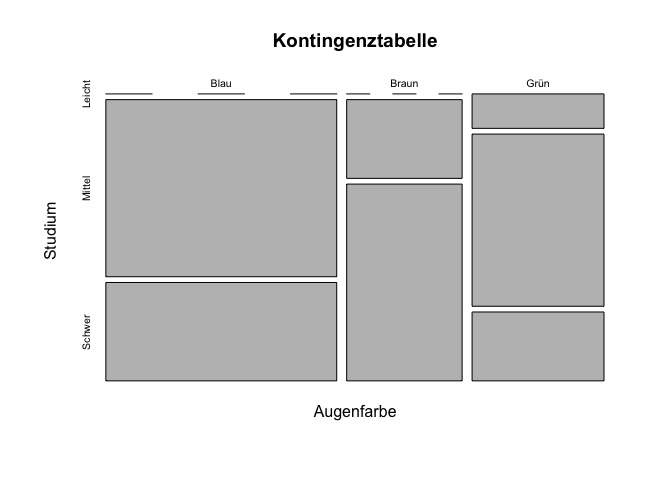
\includegraphics[width=\maxwidth]{figure/unnamed-chunk-4-1} \begin{Sinput}
surv <- as.numeric(survived)-1 # glm requires 0 / 1 not true false
\end{Sinput}
\end{Schunk}


Wie analysieren wir diese Daten? Die Response ist eindeutig nicht normal, jedoch 1/0. Das GLM ist im Grunde das gleiche wie lm (), nur dass wir die Familie angeben.

Wir werden zuerst testen, ob das überleben mit dem Alter korreliert

\begin{Schunk}
\begin{Sinput}
fmt <- glm(surv ~ age, family=binomial)
summary(fmt)
\end{Sinput}
\begin{Soutput}

Call:
glm(formula = surv ~ age, family = binomial)

Deviance Residuals: 
    Min       1Q   Median       3Q      Max  
-1.1189  -1.0361  -0.9768   1.3187   1.5162  

Coefficients:
             Estimate Std. Error z value Pr(>|z|)  
(Intercept) -0.136531   0.144715  -0.943   0.3455  
age         -0.007899   0.004407  -1.792   0.0731 .
---
Signif. codes:  0 '***' 0.001 '**' 0.01 '*' 0.05 '.' 0.1 ' ' 1

(Dispersion parameter for binomial family taken to be 1)

    Null deviance: 1414.6  on 1045  degrees of freedom
Residual deviance: 1411.4  on 1044  degrees of freedom
  (263 observations deleted due to missingness)
AIC: 1415.4

Number of Fisher Scoring iterations: 4
\end{Soutput}
\end{Schunk}

Ergebnis geplottet

\begin{Schunk}
\begin{Sinput}
plot(surv ~ age, main="only age term")
newage <- seq(min(age, na.rm=T), max(age, na.rm=T), len=100)
preds <- predict(fmt, newdata=data.frame("age"=newage), se.fit=T)
lines(newage, plogis(preds$fit), col="purple", lwd=3)
lines(newage, plogis(preds$fit-2*preds$se.fit), col="purple", lwd=3, lty=2)
lines(newage, plogis(preds$fit+2*preds$se.fit), col="purple", lwd=3, lty=2)
\end{Sinput}

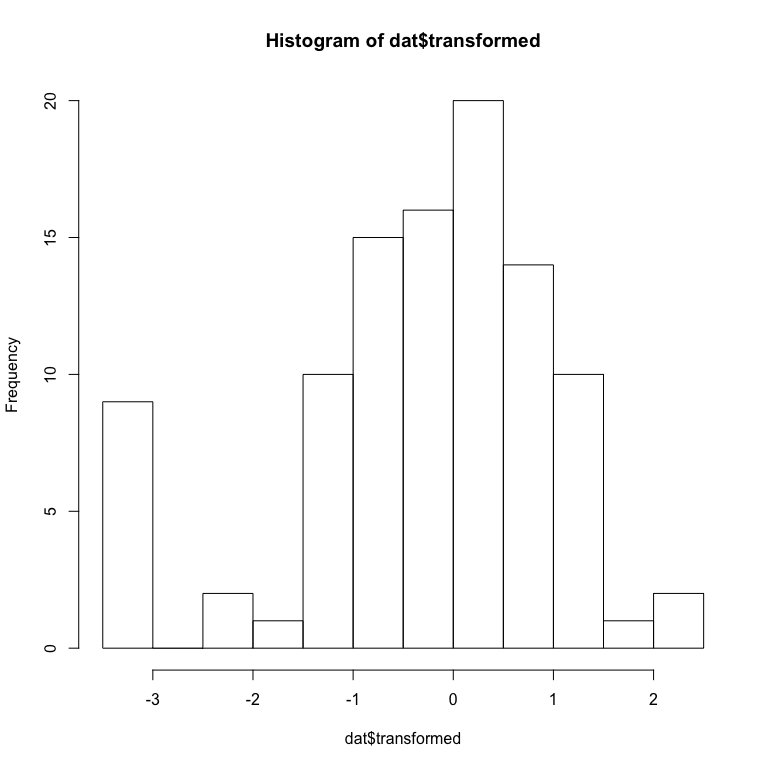
\includegraphics[width=\maxwidth]{figure/unnamed-chunk-6-1} \end{Schunk}


Nun setzen wir alle relevanten Variablen ein in:

\begin{Schunk}
\begin{Sinput}
surv <- as.numeric(survived)-1 # glm requires 0 / 1 not true false
fmt <- glm(surv ~ age  + sex + passengerClass, family=binomial)
summary(fmt)
\end{Sinput}
\begin{Soutput}

Call:
glm(formula = surv ~ age + sex + passengerClass, family = binomial)

Deviance Residuals: 
    Min       1Q   Median       3Q      Max  
-2.6399  -0.6979  -0.4336   0.6688   2.3964  

Coefficients:
                   Estimate Std. Error z value Pr(>|z|)    
(Intercept)        3.522074   0.326702  10.781  < 2e-16 ***
age               -0.034393   0.006331  -5.433 5.56e-08 ***
sexmale           -2.497845   0.166037 -15.044  < 2e-16 ***
passengerClass2nd -1.280570   0.225538  -5.678 1.36e-08 ***
passengerClass3rd -2.289661   0.225802 -10.140  < 2e-16 ***
---
Signif. codes:  0 '***' 0.001 '**' 0.01 '*' 0.05 '.' 0.1 ' ' 1

(Dispersion parameter for binomial family taken to be 1)

    Null deviance: 1414.62  on 1045  degrees of freedom
Residual deviance:  982.45  on 1041  degrees of freedom
  (263 observations deleted due to missingness)
AIC: 992.45

Number of Fisher Scoring iterations: 4
\end{Soutput}
\end{Schunk}

\subsection{ANOVA für GLM}

Wenn eine ANOVA erwünscht ist


\begin{Schunk}
\begin{Sinput}
library(car)
\end{Sinput}
\begin{Soutput}
Warning: package 'car' was built under R version 3.3.2
\end{Soutput}
\begin{Soutput}

Attaching package: 'car'
\end{Soutput}
\begin{Soutput}
The following object is masked from 'package:effects':

    Prestige
\end{Soutput}
\begin{Sinput}
Anova(fmt)
\end{Sinput}
\begin{Soutput}
Analysis of Deviance Table (Type II tests)

Response: surv
               LR Chisq Df Pr(>Chisq)    
age              31.344  1  2.161e-08 ***
sex             273.239  1  < 2.2e-16 ***
passengerClass  118.886  2  < 2.2e-16 ***
---
Signif. codes:  0 '***' 0.001 '**' 0.01 '*' 0.05 '.' 0.1 ' ' 1
\end{Soutput}
\begin{Sinput}
detach(TitanicSurvival)
\end{Sinput}
\end{Schunk}

\section{Zähldaten - Poisson's Regression}

Für Zähldaten verwenden wir den GLM mit der Poisson'schen-Fehlerverteilung. Hier sind einige Beobachtungen der Verteilung von Futterstücke an junge Vögel und ihre wahrgenommene Attraktivität.

\begin{Schunk}
\begin{Sinput}
cfc <- data.frame(
  stuecke = c(3,6,8,4,2,7,6,8,10,3,5,7,6,7,5,6,7,11,8,11,13,11,7,7,6),
  attrakt = c(1,1,1,1,1,2,2,2,2,2,3,3,3,3,3,4,4,4,4,4,5,5,5,5,5) 
)
attach(cfc)
plot(stuecke ~ attrakt)
\end{Sinput}

\includegraphics[width=\maxwidth]{figure/unnamed-chunk-72-1} \end{Schunk}

So wird der Poisson angegeben

\begin{Schunk}
\begin{Sinput}
fm <- glm(stuecke ~ attrakt, family=poisson)
summary(fm)
\end{Sinput}
\begin{Soutput}

Call:
glm(formula = stuecke ~ attrakt, family = poisson)

Deviance Residuals: 
     Min        1Q    Median        3Q       Max  
-1.55377  -0.72834   0.03699   0.59093   1.54584  

Coefficients:
            Estimate Std. Error z value Pr(>|z|)    
(Intercept)  1.47459    0.19443   7.584 3.34e-14 ***
attrakt      0.14794    0.05437   2.721  0.00651 ** 
---
Signif. codes:  0 '***' 0.001 '**' 0.01 '*' 0.05 '.' 0.1 ' ' 1

(Dispersion parameter for poisson family taken to be 1)

    Null deviance: 25.829  on 24  degrees of freedom
Residual deviance: 18.320  on 23  degrees of freedom
AIC: 115.42

Number of Fisher Scoring iterations: 4
\end{Soutput}
\end{Schunk}

Vorhersagen

\begin{Schunk}
\begin{Sinput}
newattrakt <- c(1,1.5,2,2.5,3,3.5,4,4.5,5)
preds <- predict(fm, newdata=data.frame("attrakt"=newattrakt))
plot(stuecke ~ attrakt)
lines(newattrakt, exp(preds), lwd=2, col="green")
\end{Sinput}

\includegraphics[width=\maxwidth]{figure/unnamed-chunk-74-1} \end{Schunk}

Das gleiche mit 95\% Konfidenzinterval:

\begin{Schunk}
\begin{Sinput}
preds <- predict(fm, newdata=data.frame("attrakt"=newattrakt), se.fit=T)
str(preds)
\end{Sinput}
\begin{Soutput}
List of 3
 $ fit           : Named num [1:9] 1.62 1.7 1.77 1.84 1.92 ...
  ..- attr(*, "names")= chr [1:9] "1" "2" "3" "4" ...
 $ se.fit        : Named num [1:9] 0.1459 0.1235 0.1034 0.0872 0.0775 ...
  ..- attr(*, "names")= chr [1:9] "1" "2" "3" "4" ...
 $ residual.scale: num 1
\end{Soutput}
\begin{Sinput}
plot(stuecke ~ attrakt)
lines(newattrakt, exp(preds$fit), lwd=2, col="green")
lines(newattrakt, exp(preds$fit+2*preds$se.fit), lwd=2, col="green", lty=2)
lines(newattrakt, exp(preds$fit-2*preds$se.fit), lwd=2, col="green", lty=2)
\end{Sinput}

\includegraphics[width=\maxwidth]{figure/unnamed-chunk-75-1} \begin{Sinput}
detach(cfc)
\end{Sinput}
\end{Schunk}



\section{Multinomiale Daten - multinomiale Regression}

Wenn man mehrere Optionen für die Response habt (rot, grün, blau), passt dies zu einer multinomialen Regression. Dies ist nicht im Standard-GLM-Paket. Das Standardpaket dazu wäre mlogit. Ich gebe dazu unten ein Beispiel an. Das Problem mit mlogit ist, dass es Daten in einer bestimmten Weise erfordert, d.h. dass für jede Beobachtung jede Auswahl eine einzelne Zeile ist. Zusätzlich gibt es eine Spalte, die sagt, welche Wahl getroffen wurde (ja / nein). Um mlogit verwenden zu können, müssen Sie die Daten in dieses Format umwandeln.

Wenn man die Daten nicht in diesem Format hat und nicht neu formatieren möchte, ist eine weniger leistungsstarke, aber einfacher zu bedienende Alternative die multinomiale Funktion aus dem nnet-Paket. Im Folgenden finden Sie ein Beispiel für die Verwendung dieser Funktion oder \href{http://www.ats.ucla.edu/stat/stata/dae/mlogit.htm}{hier}.

\subsection{mlogit Beispiel}



\begin{Schunk}
\begin{Sinput}
library(mlogit)
\end{Sinput}
\begin{Soutput}
Warning: package 'mlogit' was built under R version 3.3.2
\end{Soutput}
\begin{Soutput}
Warning: package 'Formula' was built under R version 3.3.2
\end{Soutput}
\begin{Soutput}
Warning: package 'maxLik' was built under R version 3.3.2
\end{Soutput}
\begin{Soutput}
Warning: package 'miscTools' was built under R version 3.3.2
\end{Soutput}
\begin{Sinput}
data("Fishing", package = "mlogit")
head(Fishing)
\end{Sinput}
\begin{Soutput}
     mode price.beach price.pier price.boat price.charter catch.beach
1 charter     157.930    157.930    157.930       182.930      0.0678
2 charter      15.114     15.114     10.534        34.534      0.1049
3    boat     161.874    161.874     24.334        59.334      0.5333
4    pier      15.134     15.134     55.930        84.930      0.0678
5    boat     106.930    106.930     41.514        71.014      0.0678
6 charter     192.474    192.474     28.934        63.934      0.5333
  catch.pier catch.boat catch.charter   income
1     0.0503     0.2601        0.5391 7083.332
2     0.0451     0.1574        0.4671 1250.000
3     0.4522     0.2413        1.0266 3750.000
4     0.0789     0.1643        0.5391 2083.333
5     0.0503     0.1082        0.3240 4583.332
6     0.4522     0.1665        0.3975 4583.332
\end{Soutput}
\end{Schunk}

Die Daten, die wir verwenden, ist ein Datenframe mit folgendem Inhalt :

\begin{enumerate}
\setlength\itemsep{-0.5em}
\item price.beach -price for beach mode

\item price.pier -price for pier mode

\item price.boat -price for private boat mode

\item price.charter -price for charter boat mode

\item catch.beach -catch rate for beach mode

\item catch.pier -catch rate for pier mode

\item catch.boat -catch rate for private boat mode

\item catch.charter -catch rate for charter boat mode

\item income - monthly income

\item mode -recreation mode choice, one of : beach, pier, boat and charter

\end{enumerate}

Wir transformieren das in ein Objekt, mit dem mlogit arbeiten kann


\begin{Schunk}
\begin{Sinput}
Fish <- mlogit.data(Fishing, varying = c(2:9), shape = "wide", choice = "mode")
\end{Sinput}
\end{Schunk}


Variation zeigt dem Modell an, dass es sich um Variablen handelt, die für die alternativen Outputs der Response spezifisch sind, z.B. der Preis des Bootes; während Variablen, die nicht variieren, unabhängig vom Output sind, z.B. Einkommen.


\begin{Schunk}
\begin{Sinput}
## a pure "conditional" model
summary(mlogit(mode ~ price + catch, data = Fish))
\end{Sinput}
\begin{Soutput}

Call:
mlogit(formula = mode ~ price + catch, data = Fish, method = "nr", 
    print.level = 0)

Frequencies of alternatives:
  beach    boat charter    pier 
0.11337 0.35364 0.38240 0.15059 

nr method
7 iterations, 0h:0m:0s 
g'(-H)^-1g = 6.22E-06 
successive function values within tolerance limits 

Coefficients :
                      Estimate Std. Error  t-value  Pr(>|t|)    
boat:(intercept)     0.8713749  0.1140428   7.6408 2.154e-14 ***
charter:(intercept)  1.4988884  0.1329328  11.2755 < 2.2e-16 ***
pier:(intercept)     0.3070552  0.1145738   2.6800 0.0073627 ** 
price               -0.0247896  0.0017044 -14.5444 < 2.2e-16 ***
catch                0.3771689  0.1099707   3.4297 0.0006042 ***
---
Signif. codes:  0 '***' 0.001 '**' 0.01 '*' 0.05 '.' 0.1 ' ' 1

Log-Likelihood: -1230.8
McFadden R^2:  0.17823 
Likelihood ratio test : chisq = 533.88 (p.value = < 2.22e-16)
\end{Soutput}
\end{Schunk}

Für jeden Outcome passt die Erhöhung der "choice" zu "price" und "catch". Daher erhalten wir die Schnittpunkte für jeden Outcome und ein Parameter pro Variable, was die Auswirkung von "price" / "choice" auf die Wahrscheinlichkeit ist, eines der 4 Ergebnisse zu wählen.

Wenn wir die Variable "income" korrelieren, ist dies anders. Das Einkommen ist nicht spezifisch für "choice" (nicht als variabel ausgewählt, als wir die Daten eingelesen haben). In diesem Fall fragen wir uns, wie sich "choice" verändert, wenn wir Menschen mit unterschiedlichen Einkommen haben. Daher erhalten wir einen Intervallwert pro Parameter und eine Schätzung, ob diese Wahl durch eine Erhöhung des Einkommens, bezogen auf die Grundlinie (Pier), beeinflusst wird.

\begin{Schunk}
\begin{Sinput}
## a pure "multinomial model"
summary(mlogit(mode ~ 0 | income, data = Fish))
\end{Sinput}
\begin{Soutput}

Call:
mlogit(formula = mode ~ 0 | income, data = Fish, method = "nr", 
    print.level = 0)

Frequencies of alternatives:
  beach    boat charter    pier 
0.11337 0.35364 0.38240 0.15059 

nr method
4 iterations, 0h:0m:0s 
g'(-H)^-1g = 8.32E-07 
gradient close to zero 

Coefficients :
                       Estimate  Std. Error t-value  Pr(>|t|)    
boat:(intercept)     7.3892e-01  1.9673e-01  3.7560 0.0001727 ***
charter:(intercept)  1.3413e+00  1.9452e-01  6.8955 5.367e-12 ***
pier:(intercept)     8.1415e-01  2.2863e-01  3.5610 0.0003695 ***
boat:income          9.1906e-05  4.0664e-05  2.2602 0.0238116 *  
charter:income      -3.1640e-05  4.1846e-05 -0.7561 0.4495908    
pier:income         -1.4340e-04  5.3288e-05 -2.6911 0.0071223 ** 
---
Signif. codes:  0 '***' 0.001 '**' 0.01 '*' 0.05 '.' 0.1 ' ' 1

Log-Likelihood: -1477.2
McFadden R^2:  0.013736 
Likelihood ratio test : chisq = 41.145 (p.value = 6.0931e-09)
\end{Soutput}
\end{Schunk}

Wenn wir die Parameterwerte interpretieren wollen, müssen wir die Response mit der relativ komplizierten Linkfunktion der multinomialen logistischen Regression zurück transformieren, siehe \href{http://en.wikipedia.org/wiki/Multinomial_logistic_regression}{hier}. Mehr Beispiele \href{http://www.inside-r.org/packages/cran/mlogit/docs/suml}{hier} und ein mlogit Tutorial findet man \href{http://cran.r-project.org/web/packages/mlogit/vignettes/Exercises.pdf}{hier}.

\subsection{mlogit Beispiel}

\begin{Schunk}
\begin{Sinput}
require(nnet)
\end{Sinput}
\end{Schunk}

Wir verwenden die ursprünglichen fishing- Daten (ohne Umformung), wie für das mlogit Beispiel siehe oben.
Und auch die gleiche Modellstruktur

\begin{Schunk}
\begin{Sinput}
## a pure "conditional" model
summary(multinom(mode ~ price.beach + price.pier + price.boat + price.charter + 
                   catch.beach + catch.pier + catch.boat + catch.charter, data = Fishing))
\end{Sinput}
\begin{Soutput}
# weights:  40 (27 variable)
initial  value 1638.599935 
iter  10 value 1259.378401
iter  20 value 1107.487082
iter  30 value 1080.109863
iter  40 value 1071.690367
final  value 1066.673017 
converged
\end{Soutput}
\begin{Soutput}
Call:
multinom(formula = mode ~ price.beach + price.pier + price.boat + 
    price.charter + catch.beach + catch.pier + catch.boat + catch.charter, 
    data = Fishing)

Coefficients:
        (Intercept)  price.beach   price.pier price.boat price.charter
pier      -7.179469 -0.002574919 -0.002574919 -0.3214320     0.3197300
boat     -13.428983  0.016175579  0.016175579 -0.5792052     0.5557474
charter  -16.149440  0.013289286  0.013289286 -0.6704588     0.6518595
        catch.beach catch.pier catch.boat catch.charter
pier       37.51200  -51.32769 -1.7835077     0.0998035
boat       58.57987  -86.66495 -0.5202275     0.3055832
charter    60.63974  -86.88573  0.3685243     0.1187109

Std. Errors:
        (Intercept) price.beach  price.pier price.boat price.charter
pier      0.5280588 0.001764405 0.001764405 0.02236164    0.02208038
boat      0.7076107 0.001779923 0.001779923 0.02771352    0.02762961
charter   0.7183116 0.001741317 0.001741317 0.02799268    0.02783368
        catch.beach catch.pier catch.boat catch.charter
pier      0.5310725  0.3762405  0.1589259     0.2567735
boat      0.6800386  0.5761398  0.5994476     0.3152429
charter   0.6516732  0.5478077  0.6099301     0.3098643

Residual Deviance: 2133.346 
AIC: 2181.346 
\end{Soutput}
\end{Schunk}
\end{appendices}


 
\end{document}
